%%
%% 研究報告用スイッチ
%% [techrep]
%%
%% 欧文表記無しのスイッチ(etitle,eabstractは任意)
%% [noauthor]
%%

%\documentclass[submit,techrep]{ipsj}
%%% <<< SES
%\documentclass[submit,techrep,noauthor]{ipsj}
\documentclass[submit,ses,noauthor]{ipsj}
%%% >>> SES


%\usepackage[dvips]{graphicx}
\usepackage[dvipdfmx]{graphicx}
\usepackage{graphicx}
\usepackage{latexsym}
\usepackage{url}
\usepackage{multirow}
\usepackage[dvipsnames]{xcolor}
\usepackage{colortbl,array}

\def\Underline{\setbox0\hbox\bgroup\let\\\endUnderline}
\def\endUnderline{\vphantom{y}\egroup\smash{\underline{\box0}}\\}
\def\|{\verb|}
%

\newcommand{\todo}[1]{\colorbox{yellow}{{\bf TODO}:}{\color{red} {\textbf{[#1]}}}}

%\setcounter{巻数}{59}%vol59=2018
%\setcounter{号数}{10}
%\setcounter{page}{1}


\begin{document}


\title{Scratchにおけるユーザの\\コンピュテーショナル・シンキングスキル\\の習熟過程の分析と習熟度予測}

\affiliate{WU}{和歌山大学システム工学部}

\author{岡本 圭悟}{Keigo Okamoto}{WU}[okamoto.keigo@g.wakayama-u.jp]
\author{伊原 彰紀}{Akinori Ihara}{WU}[ihara@wakayama-u.ac.jp]

\begin{abstract}
本研究では,Scratchにおけるユーザのコンピュテーショナル・シンキング (CT) の習熟過程に基づいて次に制作する作品でCT習熟度が向上するか否かを予測する手法を構築する.従来研究では,ユーザのCTスキルの習熟過程は十分考慮できておらず,誤って予測することがあった.本研究では,過去に制作した作品でCTスキルの使用順に基づく予測モデルを構築した結果,特定の習熟度に到達するユーザを従来手法よりも高い精度で予測することを確認した.
\end{abstract}


%
%\begin{jkeyword}
%情報処理学会論文誌ジャーナル,\LaTeX,スタイルファイル,べからず集
%\end{jkeyword}
%
%\begin{eabstract}
%This document is a guide to prepare a draft for submitting to IPSJ
%Journal, and the final camera-ready manuscript of a paper to appear in
%IPSJ Journal, using {\LaTeX} and special style files.  Since this
%document itself is produced with the style files, it will help you to
%refer its source file which is distributed with the style files.
%\end{eabstract}
%
%\begin{ekeyword}
%IPSJ Journal, \LaTeX, style files, ``Dos and Dont's'' list
%\end{ekeyword}

\maketitle

%%%%%%%%%%%%%%%%%%%%%%
%1
\section{はじめに}
%%%%%%%%%%%%%%%%%%%%%%

初等教育におけるプログラミング教材の一つとして,MITメディアラボが開発するビジュアルプログラミング言語Scratch~\cite{Resnick_2009}が利用が進み,テキストベースのプログラミングへの移行を容易にすることを実証実験により明らかにしている\cite{TCE17-Weintrop}.Scratchでは,プログラミングにおける命令処理を視覚的なブロックとして表現し,それらを組み合わせることでユーザの直感的なプログラム制作を実現している.
プログラミング学習は,プログラミングの問題に対する抽象的な分析や,その問題を解決するためのComputational Thinking(以下,CT)~\cite{Wing_2006}を身につけることが目的である.CTは,主に問題を応用可能な一般式にする抽象化,問題を一般式に当てはめて表現する実装,問題を解いて確かめる分析の3手順の反復によって習熟する.プログラミング学習を通して身につけたCTをユーザが自身で把握することは困難であるため,Morenoらはユーザが制作した作品に使用されたブロックに基づきCTを計測するDr.Scratch~\cite{Moreno_2015}を開発している.Dr.Scratchは,Scratch作品で利用されたブロックやプログラムの構造から作品の機能実装に必要な7つのCT概念(抽象化,並列,論理,同期,フロー制御,ユーザ対話性,データ表現)を定量的に計測する.表\ref{tab:analysis_method}に各CT概念の計測方法を示す.各CT概念は,作品中に使用されたブロックの種類やその数に基づいて,それぞれ0点から3点までの4段階の点数によって評価される.本研究では7つのCT概念の点数の組み合わせをCTスキルと呼ぶ.また,作品自体はそれぞれのCT概念の点数を合計した0点から21点の22段階(CTスコア)で評価する.特に,CTスコアを3つの区分(CT習熟度)に分類し,0点から7点をBasic,8点から14点をDeveloping,15点から21点をMasterとして評価している.Dr.Scratchは教育環境において有用であることが確認されている\cite{Moreno_2015}\cite{WiPSCE-Jesus}\cite{IDC2019-Troiano}.具体的には.従来研究で10歳から14歳の子供を対象にDr.Scratchの評価を受けた後のCTスコアを調査した結果,CT習熟度の3つの区分でCTスコアの向上度合いに有意な差を確認している.

%-------------------
\begin{table*}[t]
    \caption{Dr.Scratchによる7つのCT概念の評価方法~\cite{Moreno_2015}}\label{tab:analysis_method}
    \vspace{1mm}
    \centering
    \scalebox{0.83}{
        \begin{tabular}{l|c|c|c}
            \hline\hline
            \multicolumn{1}{c|}{CT概念} & 1点 & 2点 & 3点 \\ \hline 
            抽象化 & \multicolumn{1}{c|}{2つ以上のスクリプトを使用} & \multicolumn{1}{c|}{定義ブロックを使用} & \multicolumn{1}{c}{クローンブロックを使用} \\ \hline
            並列 & \begin{tabular}{c}緑の旗ブロックを2個以上使用\end{tabular} & \begin{tabular}{c}2つ以上のスクリプトを同時に\\実行する機能を実装\end{tabular} & \begin{tabular}{c}イベント動作により2つ以上の\\スクリプトを同時に実行する機能を実装\end{tabular} \\ \hline
            論理 & Ifブロックを使用 & If elseブロックを使用 & 論理演算ブロックを使用 \\ \hline
            同期 & 待機ブロックを使用 & \begin{tabular}{c}メッセージを受信すると\\プログラムを停止する機能を実装\end{tabular} & \begin{tabular}{c}指定条件を満たすまで\\プログラムを停止する処理を実装\end{tabular} \\ \hline
            フロー制御 & 2個以上の処理ブロックを連結して使用 & \begin{tabular}{c}指定回数,または回数無制限の\\繰り返しブロックを使用\end{tabular} & 指定条件までの繰り返しブロックを使用 \\ \hline
            ユーザ対話性 & 緑の旗ブロックを使用 & \begin{tabular}{c}ユーザによる入力を伴うブロックを使用\end{tabular} & \begin{tabular}{c}インタラクションを伴うブロックを使用\end{tabular} \\ \hline
            データ表現 & \begin{tabular}{c}オブジェクトの大きさや位置等のプロパティを編集\end{tabular} & 変数ブロックを使用 & リスト変数ブロックの使用 \\ \hline
        \end{tabular}
    }\
    \vspace{-2mm}
 \end{table*}
%-------------------

従来研究では,CTの習熟過程を明らかにするために,ユーザが制作した作品に使用するCTスキルの調査研究が行われている~\cite{Yang_2015}\cite{Troiano_2019}.安東ら~\cite{Ando_2021}は,ユーザのCTスキルの成長度合いを評価する方法として,ユーザが過去に制作した作品を通して使用したCT概念の経験有無に基づき,次に制作する作品のCT習熟度を予測する手法を開発した.安東らが提案する手法は,ユーザが作品制作に使用したCTスキルの使用順を考慮していないため,CTスコアが同じでも異なる習熟過程を持つユーザを誤って予測することがある.

本研究では,過去に制作した作品のCTスキルの使用順に基づいて,次に制作する作品のCT習熟度が向上するか否かを予測する手法を構築する.具体的にはユーザのCTスキルの習熟過程を離散パラメータの一様N階マルコフ連鎖によるものとして扱い,ランダムフォレストモデルとN階マルコフ連鎖モデルを
構築する.また,本研究では,2つのResearch Question (RQ) に回答する.

\begin{itemize}
\item[RQ1:]CT習熟度が向上するユーザが過去の作品で使用するCTスキルの特徴は?
\item[RQ2:]CTスキルの使用履歴に基づいて次に制作する作品のCT習熟度は予測可能か?
\end{itemize}

本研究により,学習速度の異なるユーザのCTスキル習熟過程を理解し,従来手法で誤予測していたユーザの習熟度到達予測を可能にする.

以降,\ref{sec:relate}章で従来研究を述べ,\ref{sec:chapter_3-1}章で本研究で用いるデータセットを述べる.また,\ref{sec:chapter_3-2},\ref{sec:rq2}章では設定した各RQの分析手法と結果,考察を述べ,最後に\ref{sec:conc}章で本論文をまとめる.


% %----------------------
 \begin{table*}[t]
\caption{BtoDユーザが習熟度向上の際に制作する作品のCTスコア重複数の上位3パターン}
  \label{tab:ranking-btod}
  \vspace{1mm}
  \centering
  \scalebox{0.83}{
\begin{tabular}{c|c|cccccccc}
\hline\hline
\multirow{2}{*}{順位} & \multirow{2}{*}{ユーザ数} & \multicolumn{8}{c}{CTスコア}\\ \cline{3-10} 
                    &                      & \multicolumn{1}{c|}{抽象化}  & \multicolumn{1}{c|}{並列} & \multicolumn{1}{c|}{論理} & \multicolumn{1}{c|}{同期} & \multicolumn{1}{c|}{フロー制御} & \multicolumn{1}{c|}{ユーザ対話性} & \multicolumn{1}{c|}{データ表現} & 合計 \\ 
                    \hline
1                   & 291                  & \multicolumn{1}{c|}{1} & \multicolumn{1}{c|}{2} & \multicolumn{1}{c|}{0} & \multicolumn{1}{c|}{1} & \multicolumn{1}{c|}{2} & \multicolumn{1}{c|}{2} & \multicolumn{1}{c|}{1} & 9  \\ \hline
2                   & 227                  & \multicolumn{1}{c|}{1} & \multicolumn{1}{c|}{2} & \multicolumn{1}{c|}{0} & \multicolumn{1}{c|}{0} & \multicolumn{1}{c|}{2} & \multicolumn{1}{c|}{2} & \multicolumn{1}{c|}{1} & 8  \\ \hline
3                   & 154                  & \multicolumn{1}{c|}{1} & \multicolumn{1}{c|}{1} & \multicolumn{1}{c|}{0} & \multicolumn{1}{c|}{1} & \multicolumn{1}{c|}{2} & \multicolumn{1}{c|}{2} & \multicolumn{1}{c|}{1} & 8  \\ 
\hline
\end{tabular}
}
% \end{table*}
% %----------------------
% \begin{table*}[t]
  \vspace{1mm}
\caption{DtoMユーザが習熟度向上の際に制作する作品のCTスコア重複数の上位3パターン}
  \label{tab:ranking-dtom}
  \vspace{1mm}
  \centering
  \scalebox{0.83}{ 
\begin{tabular}{c|c|cccccccc}
\hline\hline
\multirow{2}{*}{順位} & \multirow{2}{*}{ユーザ数} & \multicolumn{8}{c}{CTスコア}\\ \cline{3-10} 
                    &                      & \multicolumn{1}{c|}{抽象化} & \multicolumn{1}{c|}{並列} & \multicolumn{1}{c|}{論理} & \multicolumn{1}{c|}{同期} & \multicolumn{1}{c|}{フロー制御} & \multicolumn{1}{c|}{ユーザ対話性} & \multicolumn{1}{c|}{データ制御} & 合計 \\ \hline
1                   & 112                  & \multicolumn{1}{c|}{3} & \multicolumn{1}{c|}{3} & \multicolumn{1}{c|}{3} & \multicolumn{1}{c|}{3} & \multicolumn{1}{c|}{3} & \multicolumn{1}{c|}{2} & \multicolumn{1}{c|}{2} & 19  \\ \hline
2                   & 84                  & \multicolumn{1}{c|}{1} & \multicolumn{1}{c|}{3} & \multicolumn{1}{c|}{3} & \multicolumn{1}{c|}{2} & \multicolumn{1}{c|}{2} & \multicolumn{1}{c|}{2} & \multicolumn{1}{c|}{2} & 15  \\ \hline
3                   & 74                  & \multicolumn{1}{c|}{1} & \multicolumn{1}{c|}{3} & \multicolumn{1}{c|}{3} & \multicolumn{1}{c|}{3} & \multicolumn{1}{c|}{2} & \multicolumn{1}{c|}{2} & \multicolumn{1}{c|}{2} & 16  \\ \hline
\end{tabular}
}
 \vspace{-5mm}
\end{table*}


%%%%%%%%%%%%%%%%%%%%%%
\section{従来研究}\label{sec:relate}
%%%%%%%%%%%%%%%%%%%%%%

Scratchにおけるユーザのプログラミング能力の成長に関する研究が多数発表されている~\cite{Yang_2015}\cite{Troiano_2019}\cite{Ando_2021}\cite{Troiano_2019-2}\cite{ICSE16_Aivalglou}\cite{OEUC10-Kafai}\cite{Troiano_2020}.Yangら~\cite{Yang_2015}やRoblesら~\cite{Robles_2017}の研究では,Scratchのユーザは作品制作を重ねていく過程で使用するブロックの種類数が増加し,特にリミックス(他のユーザが制作した作品の再利用)しているユーザは増加することを確認した.Troianoら~\cite{Troiano_2019}の研究では,13歳から14歳の生徒が作品制作する過程で並列,論理,同期の点数が高くなる生徒が多いが,抽象化やデータ表現の点数が高くなる生徒が少ないことを確認している.

安東らは,ユーザのCTスキルの成長度合いを評価する方法として,ユーザが過去に制作した作品のCTスキルに基づいて,次に制作する作品のCT習熟度を予測する手法を開発している~\cite{Ando_2021}.事前分析としてユーザが特定の習熟度に到達するまでに制作した作品で使用されるCT概念の特徴を分析した.分析の結果,ユーザは同程度のCTスコアの作品を連続して複数回制作することで習熟度が向上することを明らかにした.
%特に,習熟度Developingのオリジナル作品を制作するまでに,ユーザは連続してBasicやDevelopingの作品を制作することが多く,Masterの作品を制作することは少ない,習熟度Masterのオリジナル作品を制作するユーザの数は少なく,Masterの作品を連続して制作することは少ない.また,
ユーザが過去に制作した作品のCT概念の経験有無に基づき,ユーザが次に制作する作品が特定の習熟度(DevelopingまたはMaster)以上の評価を得るかを予測するモデルを構築した.説明変数はユーザが過去に作品制作で使用した7つのCT概念の0点から3点の獲得有無を用い,モデルの構築にはランダムフォレストを用いている.その結果,DevelopingやMasterに到達するユーザを高い精度で予測することができたが,特定の習熟度に到達するまでに制作したCTスキルの使用順は考慮していない.

本研究では事前分析として,ユーザが初めてDeveloping以上またはMasterに到達した作品のCTスキルを調査する.表\ref{tab:ranking-btod},表\ref{tab:ranking-dtom}は,紙面の都合上,同じ概念を使用して制作した作品数の多いそれぞれ3パターンのみを示す.Developingに到達する作品の中で,並列,同期の点数が異なる.また,Masterに到達した作品は合計点数の分散がDevelopingに到達する作品に比べて大きく,抽象化,同期,フロー制御の点数が異なる.このように,特定の習熟度に到達した作品の中でも使用されるCTスキルが異なるため,それまでに制作した作品に使用したCTスキルも異なることが示唆される.特定の習熟度に到達するまでに制作した作品に使用されたCTスキルも異なることが示唆される.本研究では,特定の習熟度に到達するまでの過程で使用されるCTスキル,および各CTスキルを用いた作品制作数を明らかにし,CTスキルの成長パターンの理解を研究の狙いとする.

%%%%%%%%%%%%%%%%%%%%%%
\section{データセット}\label{sec:chapter_3-1}
%%%%%%%%%%%%%%%%%%%%%%
本研究では,従来研究~\cite{Ando_2021}と同様に,2019年1月3日から2020年1月3日までの間に初めて作品公開を行い,分析対象期間中に20件以上の作品を制作し,且つ全ての作品でDr.ScratchでCTスコアの計測が成功したユーザ6,323人(各人20作品,合計126,460作品)を分析対象とする.本研究では,ユーザが一度でも特定の習熟度を満たす作品を制作すれば当該習熟度に到達したと判断し,リミックスによって制作された作品は習熟度に到達したと判断しない.分析対象のユーザの中で,20番目の作品を制作するまでにBasicからDeveloping以上に向上したユーザ(BtoDユーザ)3,125人,DevelopingからMasterに向上したユーザ(DtoMユーザ)1,196人を確認した.また,20作品を制作する過程で,BasicからDevelopingに向上し,さらにDevelopingからMasterに向上するユーザもいるため,BtoDユーザとDtoMユーザの間には重複がある.

%%%%%%%%%%%%%%%%%%%%%%
\section{RQ1:CT習熟度が向上するユーザが過去の作品で使用するCTスキルの特徴は?}\label{sec:chapter_3-2}
%%%%%%%%%%%%%%%%%%%%%%
\vspace{-2mm}
\subsection{分析手法}\label{sec:rq1-approach}

本研究では,ユーザがDeveloping以上の作品,またはMasterの作品を制作するために,過去に制作した作品で使用したCTスコアの系列(CTパス)を追跡する.
図\ref{fig:digraph}は2人のBtoDユーザのCTパスの概略図を示す.ユーザAはDevelopingの作品を制作するまでに3作品($A_1$,$A_2$,$A_3$),ユーザBは2作品($B_1$,$B_2$)を制作している.図中には各作品をノードで表現し,ノード内のレーダーチャートは,CT概念7種類のスコアを示す.レーダーチャートの最外側がCTスコア3点,最内側が0点とする.ノード間のエッジはユーザによる作品の制作順序を表す.ユーザAの最初の作品($A_1$)は,全てのCTスコアが0点,2番目の作品($A_2$)はフロー制御,ユーザ対話性,データ表現の概念を1点を獲得している.3番目の作品($A_3$)ではユーザ対話性と論理の概念で2点を獲得し,4番目で習熟度Developingに到達している.過去の作品でリミックス作品を制作した場合も,ユーザにとっては学習の一部とみなし,習熟過程で制作されたリミックス作品はCTパスに含める.


RQ1では,特定の習熟度に到達するまでの過程で使用したCTスキル,および各CTスキルを用いたユーザの作品制作数を明らかにする.具体的には,特定の習熟度に到達するまでに,多くのユーザが共通して使用するCTスキルを追跡する.図\ref{fig:digraph}の例では,2人のユーザが特定の習熟度に到達するまでにノード$A_2$とノード$B_1$,ノード$A_3$とノード$B_2$の作品でCTスキルが共通していることがわかる.本手法により特定の習熟度に到達するまでの過程で使用されるCTスキルの特徴を明らかにできる.


%---------------------
\begin{figure}[t]
    \centering
    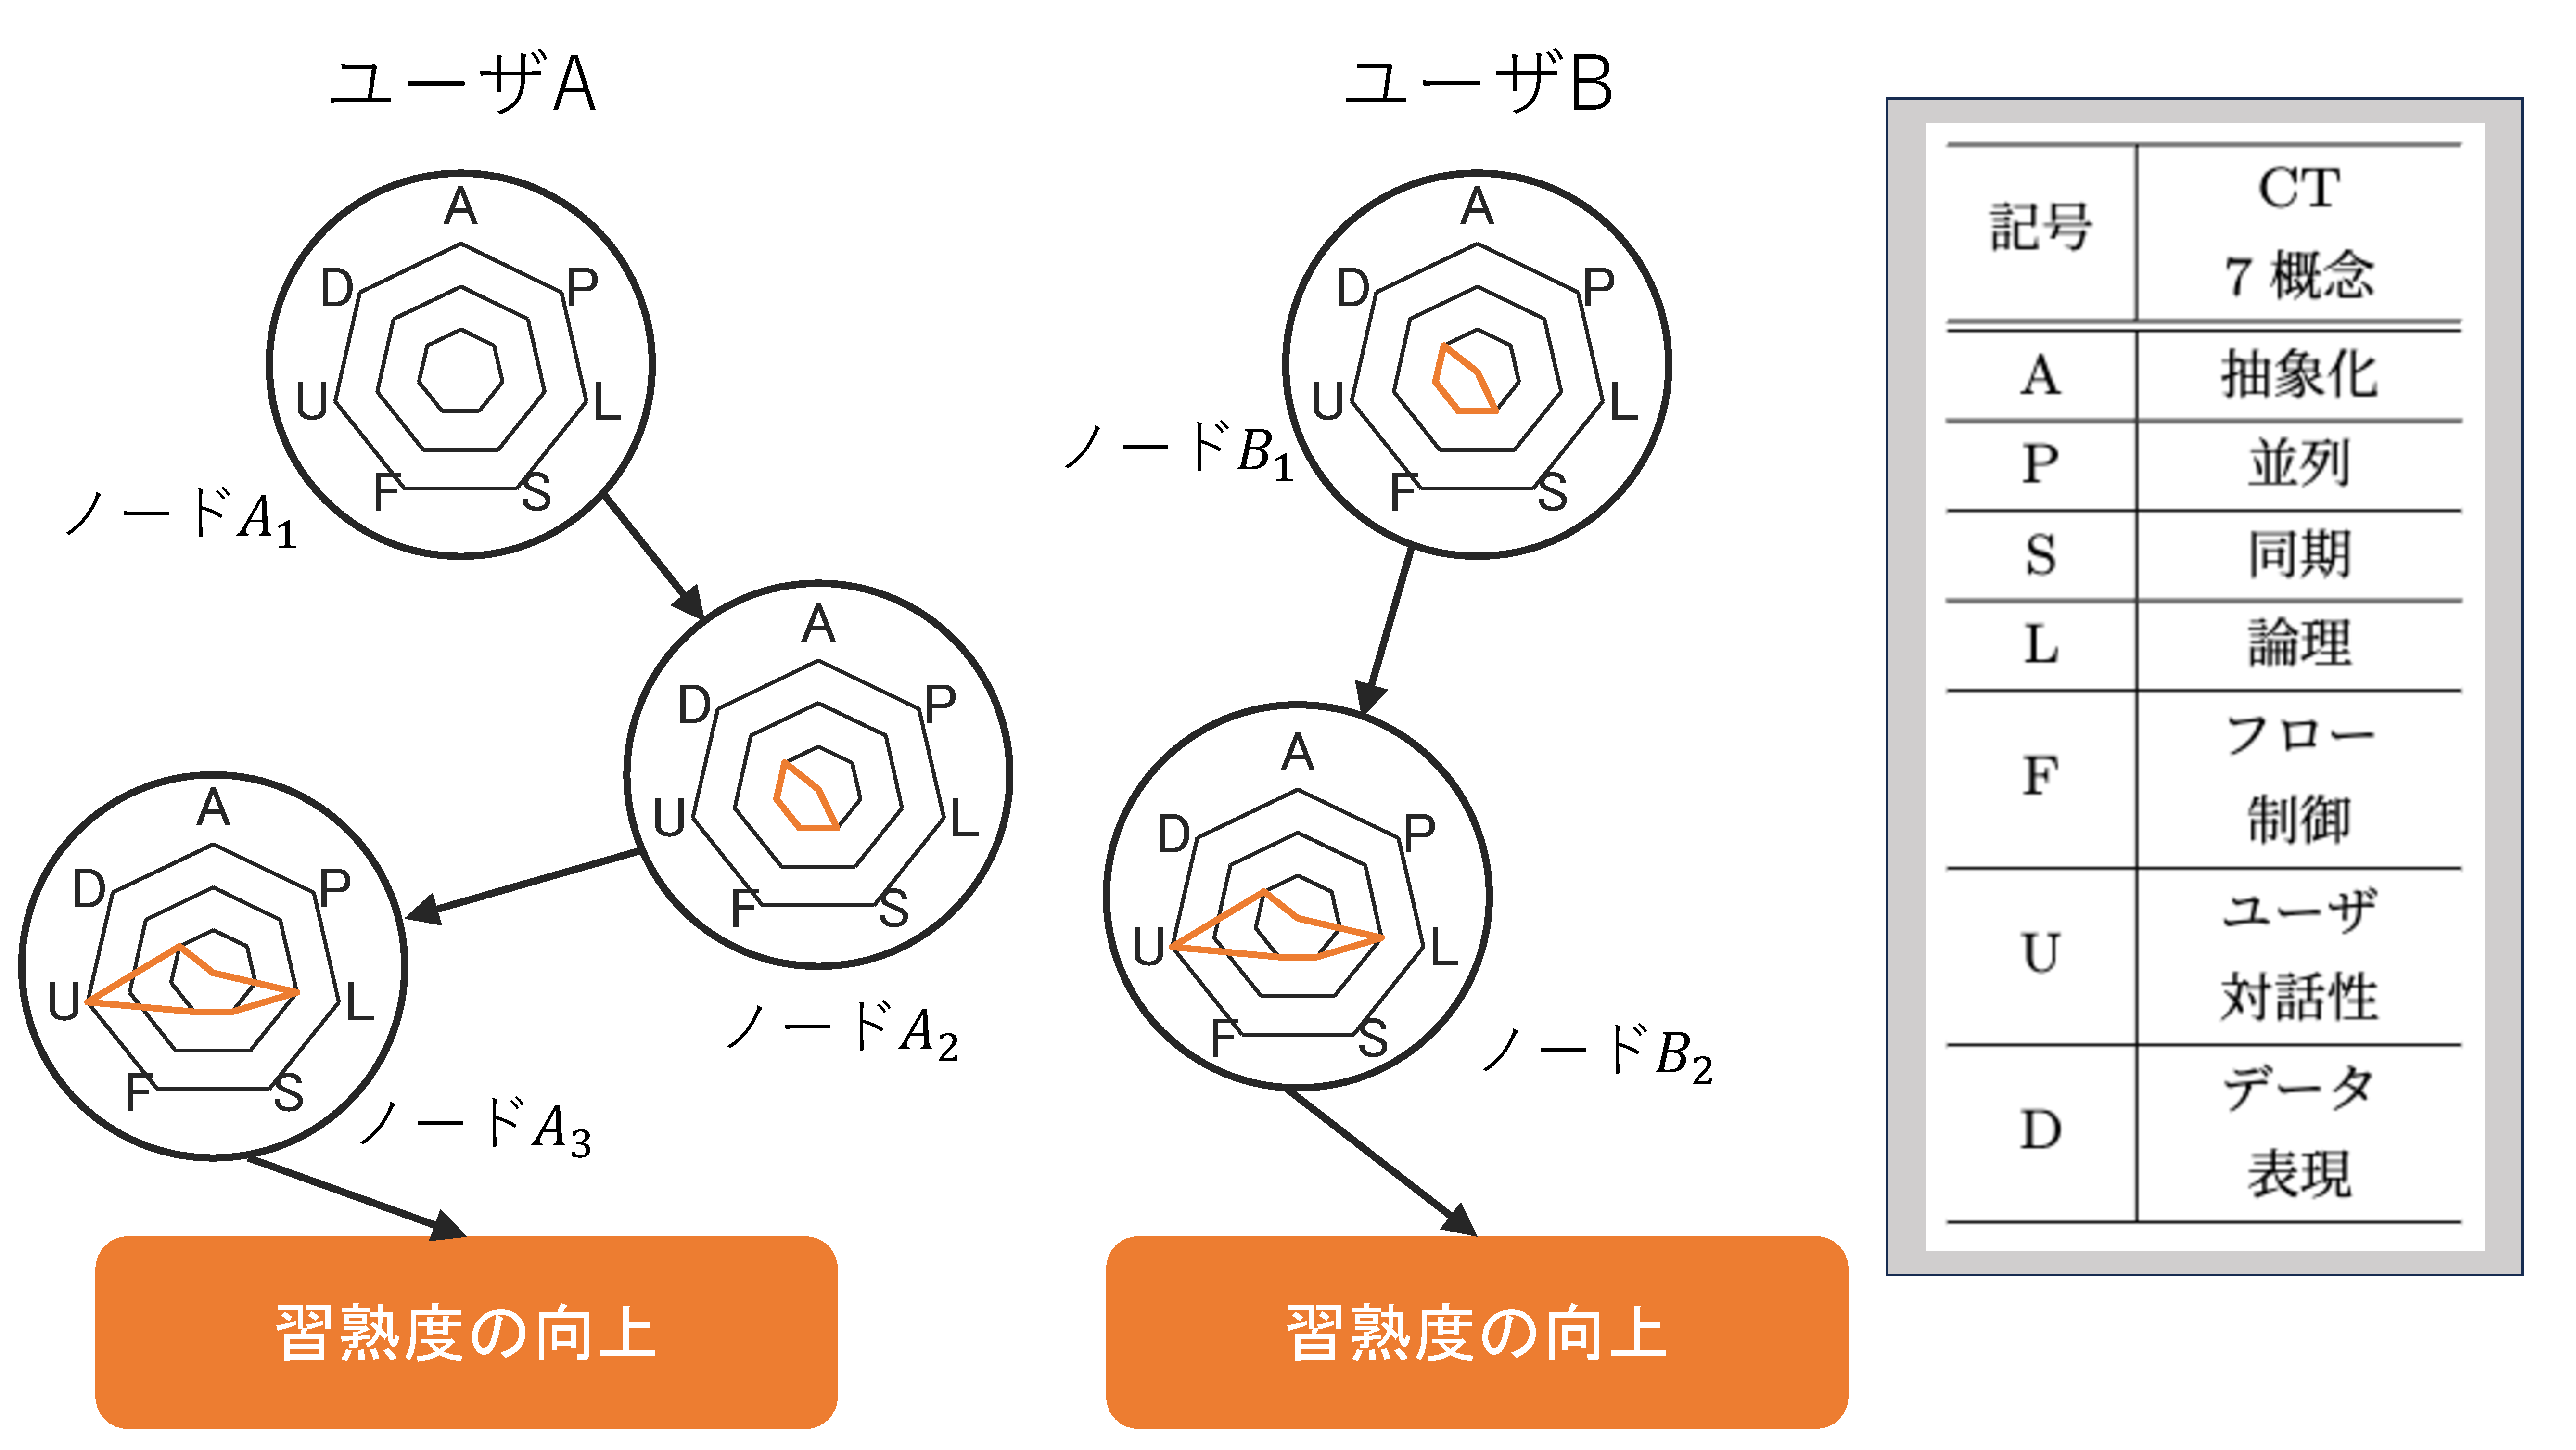
\includegraphics[width=1.0\linewidth]{Okamoto_fig/graph.pdf}
    \caption{BtoDユーザ2人のCTパスの概略図}
    \label{fig:digraph}
    \vspace{-4mm}
\end{figure}

\vspace{-2mm}
\subsection{分析結果}\label{sec:3-analysis}

\subsubsection{ユーザが使用するCTスキルの共通性の分析}\label{subsec:path-analysis}

本分析では,ユーザが制作した作品と同じCTスキルを使用して制作された他のユーザとの作品数(重複数)を分析することで,多くのユーザが特定の習熟度に到達するまでに使用したCT概念の順番や制作した作品数などの到達過程を明らかにする.従来研究\cite{Ando_2021}においてユーザが特定の習熟度に到達するまでに共通のCTを使用することが明らかにされている.当該CTを習得することが必要であるとは限らないが,習得することで学習を効率化できることが示唆される.重複数の算出方法を図\ref{fig:digraph}の例で説明すると,ユーザAは制作した3つの作品のうち,$A_1$はユーザBのいずれの作品ともCTスキルが共通していないため重複数は1,$A_2$は$B_1$と共通のCTスキルを使用しているため重複数は2,$A_3$は$B_2$と共通のCTスキルを使用しているため重複数は2となり,ユーザAが制作した作品のCTスキルの平均重複数は1.67 ($=(1 + 2 + 2) / 3$)となる.

図\ref{fig:dupli-mean}は,全てのユーザのCTスキルの重複数を習熟度別に算出した分布を箱ひげ図で示す.BtoDユーザとDtoMユーザのCTパスの重複数は,それぞれ中央値が10.5(平均値35.8),中央値が1.0(平均値2.4)であった.Mann-Whitney U検定(p値$<$0.05)を適用した結果,BtoDユーザとDtoMユーザのCTスキルの重複数に統計的有意差が見られた.したがって,BtoDユーザがDeveloping以上に到達するまでに制作した作品は,共通して使用するCTスキルが存在すると示唆される.

%---------------------
\begin{figure}[t]
	\centering
	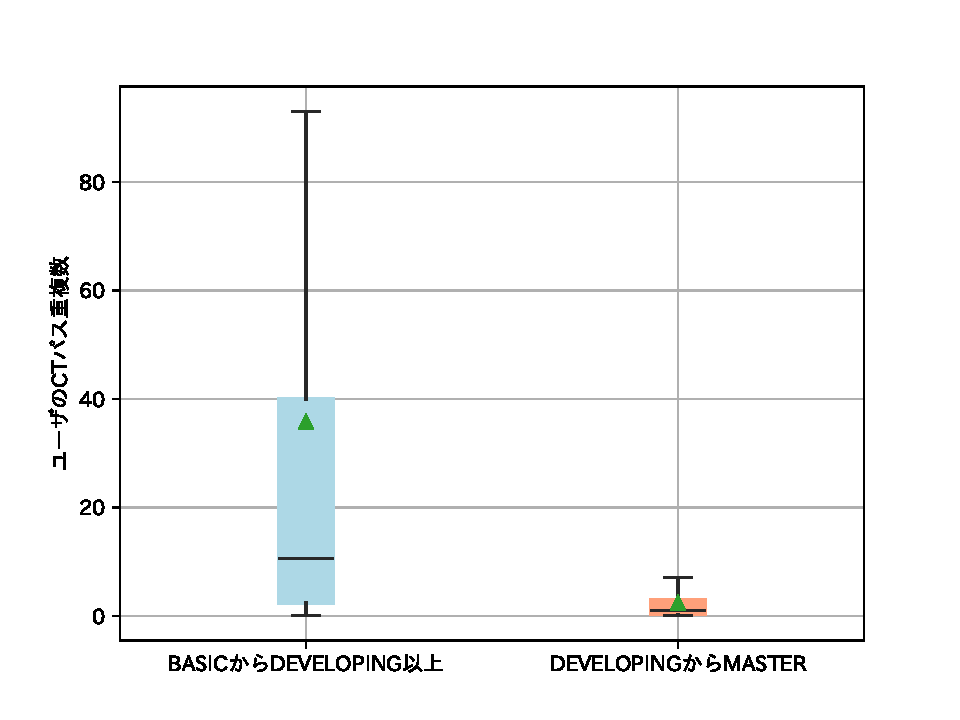
\includegraphics[width=0.8\linewidth]{Okamoto_fig/dupli-all.pdf}
	\caption{各習熟度に到達したユーザのCTスキル重複数の分布}
	\label{fig:dupli-mean}
\end{figure}
% %---------------------

\subsubsection{制作過程で使用するCTスキルの分析}\label{subsec:ct-analysis}

%-----------------------
\begin{table*}[t]
  \begin{minipage}[t]{0.45\linewidth} % 0.5\linewidthはページ幅の半分に相当
    \centering
    \caption{BtoDユーザが習熟度向上までに制作した\\作品数毎の代表CTパス}
    \label{tab:split-ct-btod}
    \vspace{1mm}
      \scalebox{0.85}{ 
  \begin{tabular}{c|l|c}
    \hline\hline
    作品数 & 代表CTパス & ユーザの割合\\
    \hline
    1 & \texttt{\large{A}} & 17\%(10/58) \\
    \hline
    2 & \texttt{\large{\textcolor{Green}{BB}}} & 43\%(18/42) \\
    \hline
    3 & \texttt{\large{\textcolor{Green}{BBB}}} & 40\%(13/33) \\
    \hline
    4 & \texttt{\large{ACDE}} & 28\%(9/32) \\
    \hline
    5 & \texttt{\large{\textcolor{Green}{F}GH\textcolor{Green}{F}I}} & 33\%(6/18) \\
    \hline
    6 & \texttt{\large{J\textcolor{Green}{B}KLJM}} & 20\%(2/10) \\
    \hline
    7 & \texttt{\large{\textcolor{Green}{FFFFFFF}}} & 35\%(6/17)  \\
    \hline
    8 & \texttt{\large{JJJJJJJM}} & 40\%(4/10) \\
    \hline
    9 & \texttt{\large{\textcolor{blue}{NNN}H\textcolor{Green}{B}KH\textcolor{Green}{J}M}} & 17\%(2/12) \\
    \hline
    10 & \texttt{\large{\textcolor{Green}{BBBBBBBBB}O}} & 29\%(2/7) \\
    \hline
    11 & \texttt{\large{\textcolor{blue}{NNNNNNNN}P\textcolor{Green}{B}I}} & 33\%(1/3) \\
    \hline
    12 & \texttt{\large{\textcolor{blue}{NNNNNNNNNNNN}}} & 27\%(3/11) \\
    \hline
    13 & \texttt{\large{\textcolor{blue}{LLLLLLLLLLLQ}R}} & 50\%(2/4) \\
    \hline
    14 & \texttt{\large{N\textcolor{Green}{B}S\textcolor{blue}{N}\textcolor{Green}{B}S\textcolor{blue}{N}\textcolor{Green}{B}S\textcolor{blue}{N}\textcolor{Green}{B}S\textcolor{blue}{N}\textcolor{Green}{B}}} & 50\%(2/4) \\
    \hline
    15 & \texttt{\large{\textcolor{blue}{QQQQQQQQQQQQQQ}T}} & 25\%(4/16) \\
    \hline
    16 & \texttt{\large{UO\textcolor{blue}{Q}VWUO\textcolor{blue}{Q}VWUO\textcolor{blue}{Q}VX\textcolor{Green}{B}}} & 33\%(1/3) \\
    \hline
    17 & \texttt{\large{CYACYACYACYACYACZ}} & 50\%(2/4) \\
    \hline
    18 & \textcolor{blue}{\texttt{\large{NNNNNNNNNNNNNNNNNN}}} & 40\%(2/5) \\
    \hline
  \end{tabular}
  }
  \end{minipage}%
  \begin{minipage}[t]{0.5\linewidth}
    \centering
    \caption{代表CTパスの記号とCT概念の対応表}
    \label{tab:dict-btod}
    \vspace{7mm}
      \scalebox{0.85}{ 
      \begin{tabular}{c|c|cccccccc}
\hline\hline
\multirow{2}{*}{記号} & \multicolumn{1}{l|}{\multirow{2}{*}{\small{リミックス}}} & \multicolumn{8}{c}{CTスコア}  \\ \cline{3-10} 
                    & \multicolumn{1}{l|}{}                       & \multicolumn{1}{c|}{A} & \multicolumn{1}{c|}{P} & \multicolumn{1}{c|}{L} & \multicolumn{1}{c|}{S} & \multicolumn{1}{c|}{F} & \multicolumn{1}{c|}{U} & \multicolumn{1}{c|}{D} & 合計 \\ \hline 
\texttt{\large{A}}                   & 0                                           & \multicolumn{1}{c|}{0} & \multicolumn{1}{c|}{0} & \multicolumn{1}{c|}{0} & \multicolumn{1}{c|}{0} & \multicolumn{1}{c|}{1} & \multicolumn{1}{c|}{1} & \multicolumn{1}{c|}{1} & 3  \\ \hline
\rowcolor{Green!30}%
\texttt{\large{B}}                   & 0                                           & \multicolumn{1}{c|}{1} & \multicolumn{1}{c|}{1} & \multicolumn{1}{c|}{0} & \multicolumn{1}{c|}{1} & \multicolumn{1}{c|}{2} & \multicolumn{1}{c|}{1} & \multicolumn{1}{c|}{1} & 7  \\ \hline
\texttt{\large{C}}                   & 0                                           & \multicolumn{1}{c|}{0} & \multicolumn{1}{c|}{0} & \multicolumn{1}{c|}{0} & \multicolumn{1}{c|}{0} & \multicolumn{1}{c|}{0} & \multicolumn{1}{c|}{0} & \multicolumn{1}{c|}{0} & 0  \\ \hline
\rowcolor{Green!30}%
\texttt{\large{F}}                   & 0                                           & \multicolumn{1}{c|}{1} & \multicolumn{1}{c|}{1} & \multicolumn{1}{c|}{0} & \multicolumn{1}{c|}{0} & \multicolumn{1}{c|}{2} & \multicolumn{1}{c|}{1} & \multicolumn{1}{c|}{1} & 6  \\ \hline
\texttt{\large{J}}                   & 0                                           & \multicolumn{1}{c|}{0} & \multicolumn{1}{c|}{0} & \multicolumn{1}{c|}{0} & \multicolumn{1}{c|}{0} & \multicolumn{1}{c|}{2} & \multicolumn{1}{c|}{2} & \multicolumn{1}{c|}{1} & 5  \\ \hline
\rowcolor{blue!30}%
\texttt{\large{L}}                   & 0                                           & \multicolumn{1}{c|}{0} & \multicolumn{1}{c|}{0} & \multicolumn{1}{c|}{0} & \multicolumn{1}{c|}{1} & \multicolumn{1}{c|}{1} & \multicolumn{1}{c|}{2} & \multicolumn{1}{c|}{1} & 5  \\ \hline
\rowcolor{blue!30}%
\texttt{\large{N}}                   & 0                                           & \multicolumn{1}{c|}{0} & \multicolumn{1}{c|}{0} & \multicolumn{1}{c|}{0} & \multicolumn{1}{c|}{0} & \multicolumn{1}{c|}{2} & \multicolumn{1}{c|}{1} & \multicolumn{1}{c|}{1} & 4  \\ \hline
\texttt{\large{O}}                   & 0                                           & \multicolumn{1}{c|}{1} & \multicolumn{1}{c|}{1} & \multicolumn{1}{c|}{0} & \multicolumn{1}{c|}{1} & \multicolumn{1}{c|}{1} & \multicolumn{1}{c|}{1} & \multicolumn{1}{c|}{1} & 6  \\ \hline
\rowcolor{blue!30}%
\texttt{\large{Q}}                   & 0                                           & \multicolumn{1}{c|}{1} & \multicolumn{1}{c|}{0} & \multicolumn{1}{c|}{0} & \multicolumn{1}{c|}{0} & \multicolumn{1}{c|}{1} & \multicolumn{1}{c|}{2} & \multicolumn{1}{c|}{1} & 5  \\ \hline
\texttt{\large{S}}                   & 0                                           & \multicolumn{1}{c|}{1} & \multicolumn{1}{c|}{0} & \multicolumn{1}{c|}{0} & \multicolumn{1}{c|}{1} & \multicolumn{1}{c|}{1} & \multicolumn{1}{c|}{2} & \multicolumn{1}{c|}{1} & 6  \\ \hline
\texttt{\large{U}}                   & 1                                           & \multicolumn{1}{c|}{3} & \multicolumn{1}{c|}{3} & \multicolumn{1}{c|}{3} & \multicolumn{1}{c|}{3} & \multicolumn{1}{c|}{3} & \multicolumn{1}{c|}{2} & \multicolumn{1}{c|}{3} & 20 \\ \hline
\texttt{\large{V}}                   & 1                                           & \multicolumn{1}{c|}{2} & \multicolumn{1}{c|}{3} & \multicolumn{1}{c|}{2} & \multicolumn{1}{c|}{3} & \multicolumn{1}{c|}{3} & \multicolumn{1}{c|}{1} & \multicolumn{1}{c|}{2} & 16 \\ \hline
\texttt{\large{W}}                   & 1                                           & \multicolumn{1}{c|}{1} & \multicolumn{1}{c|}{3} & \multicolumn{1}{c|}{0} & \multicolumn{1}{c|}{2} & \multicolumn{1}{c|}{2} & \multicolumn{1}{c|}{1} & \multicolumn{1}{c|}{2} & 11 \\ \hline
\texttt{\large{Y}}                   & 0                                           & \multicolumn{1}{c|}{0} & \multicolumn{1}{c|}{0} & \multicolumn{1}{c|}{0} & \multicolumn{1}{c|}{1} & \multicolumn{1}{c|}{1} & \multicolumn{1}{c|}{1} & \multicolumn{1}{c|}{1} & 4  \\ \hline
\end{tabular}
}
  \end{minipage}
  \vspace{-4mm}
\end{table*}
%-----------------------

\noindent\textbf{BtoDユーザの分析:} 表\ref{tab:ranking-btod}に習熟度Developing到達時の作品で使用されたCTスキルの3パターンを示しているが,Developingに到達した作品のCTスキルごとに,それまでに制作された全ての作品のCTスキルを述べることは紙面の都合上,困難である.したがって,本論文では,表\ref{tab:ranking-btod}で最も多くのユーザ(291人)がDevelopingに到達するまでに,各ユーザが制作過程で使用したCTスキルを分析する.表\ref{tab:split-ct-btod}は,Developingに到達するまでに制作した作品数別に,最も多いCTパス(代表CTパス)を示す.代表CTパスに示す記号列は,左から右に行くほど新しい作品で使用したCTスコアを示し,各記号は紙面の都合上,複数回獲得されているCTスコアのみ表\ref{tab:dict-btod}に示す.例えば,作品数2の代表CTパスはBBであるため,ユーザは抽象化,並列,同期,ユーザ対話性,データ表現で1点,フロー制御で2点の2作品を連続で制作したのち,Developingに到達したことを示す.

\noindent\textbf{知見1: 過去に制作した作品数が多いユーザと少ないユーザはそれぞれ類似するCT概念を使用する.}

代表CTパスから,並列で1点を獲得する記号BとF(表\ref{tab:split-ct-btod}の緑文字)はDevelopingに到達するまでに制作した作品数が比較的少ないユーザで使用され,Scratch開始時点からCTを理解していることが示唆される.一方で,合計CTスコアが低い(フロー制御,ユーザ対話性,データ表現を1点ずつ獲得する)記号NやLやQ(表\ref{tab:split-ct-btod}の青文字)はDevelopingに到達するまでに制作した作品が多いユーザが使用している.したがって,Developingまでに制作する作品数の少ないユーザは並列処理を使用し,制作する作品数の多いユーザは並列処理を使用しない傾向にあることが示唆される.

\noindent\textbf{知見2: 同じCT概念を繰り返し獲得することで習熟度を向上しているユーザが多い}.

代表CTパスには,同じCTスキルの作品を繰り返すことで習熟度を向上しているユーザを確認できる.具体的には,作品数14や16の代表CTパスは,それぞれNBSやUOQVのCT概念を繰り返して習熟度を向上している.同じCTスキルを使用している理由には,異なる種類のブロックを使用せずに,類似する作品の制作を繰り返しているためDevelopingに到達する作品を制作できずにいることが示唆される.本結果は従来研究\cite{Yang_2015}が成長に従いブロックの種類数が増加するという結果を裏付けている.また,作品数16の代表CTパスでは,CTスコアの高い作品をリミックスした作品(記号\texttt{\large{U,V,W}})を制作することで習熟度が向上していることが示唆され,従来研究\cite{Yang_2015}の結果を裏付ける.

\noindent\textbf{DtoMユーザの分析: }BtoDユーザの分析結果と同様に,本論文では,表\ref{tab:ranking-dtom}で最も多くのユーザ(112人)が獲得したCTスコアに到達するまでに,各ユーザが制作過程で使用したCTスキルを分析する.表\ref{tab:split-ct-dtom}は,習熟度Masterに到達するまでに制作した作品数別の代表CTパスを示す.一度しか獲得していないCTスコアは抽象化して * として示す.また,表\ref{tab:split-ct-dtom}で示す記号は表\ref{tab:split-ct-btod}で示した記号とは別のCTスコアを示す.代表CTパスの各記号は表\ref{tab:dict-dtom}に示すCTスコアの作品を制作したことを示す.

\noindent\textbf{知見3: BtoDユーザに比べて多様なCTパスを経由して習熟度Masterの作品を制作している.}

DtoMユーザはBtoDユーザに比べて共通して制作する作品が少ないため,DtoMユーザはより多様なCTパスを経てMasterの作品を制作することが示唆される.
また,作品の制作数が11以上のユーザは作品数16と18を除いた全てのCTパスで記号M,c,d,Q,f,g,O(表\ref{tab:split-ct-dtom}の青文字))のCTスキルを獲得している.これら作品のCTスコアは平均8点とMasterに到達する点数(15点以上)に比べて低く,多数の作品制作を繰り返したのちにMasterに到達している.

%---------------------
\begin{table*}[t]
  \begin{minipage}[t]{0.45\linewidth} % 0.5\linewidthはページ幅の半分に相当
    \centering
    \caption{習熟度向上までに制作した作品数毎の代表CTパス}
    \label{tab:split-ct-dtom}
    \vspace{1mm}
      \scalebox{0.85}{ 
  \begin{tabular}{c|l|c}
    \hline    \hline
    作品数 & 代表CTパス & ユーザの割合\\
    \hline
    1 & \texttt{\large{A}} & 29\%(2/7) \\
    \hline
    2 & \texttt{\large{BB}} & 29\%(2/7) \\
    \hline
    3 & \texttt{\large{CDE}} & 20\%(1/5) \\
    \hline
    4 & \texttt{\large{FFGH}} & 25\%(1/4) \\
    \hline
    5 & \texttt{\large{IJKLK}} & 100\%(1/1) \\
    \hline
    6 & \texttt{\large{\textcolor{blue}{M}NOP\textcolor{blue}{Q}R}} & 50\%(1/2) \\
    \hline
    7 & \texttt{\large{SSTUVWX}} & 100\%(4/4)  \\
    \hline
    8 & \texttt{\large{YZZaaaZ*}} & 100\%(1/1) \\
    \hline
    9 & \texttt{\large{*****\textcolor{blue}{QQ}bb}} & 29\%(2/7) \\
    \hline
    10 & \texttt{\large{JJ*b*bbbbb}} & 40\%(2/5) \\
    \hline
    11 & \texttt{\large{\textcolor{blue}{Mcd}e\textcolor{blue}{Qfg}*hi\textcolor{blue}{O}}} & 29\%(2/7) \\
    \hline
    12 & \texttt{\large{\textcolor{blue}{Mcd}je\textcolor{blue}{Qfg}khi\textcolor{blue}{O}}} & 13\%(3/24) \\
    \hline
    13 & \texttt{\large{\textcolor{blue}{Mcd}je\textcolor{blue}{Q}c\textcolor{blue}{fg}bZi\textcolor{blue}{O}}} & 20\%(2/10) \\
    \hline
    14 & \texttt{\large{\textcolor{blue}{Mcd}je\textcolor{blue}{Qfg}**k*i\textcolor{blue}{O}}} & 29\%(2/7) \\
    \hline
    15 & \texttt{\large{\textcolor{blue}{Mcd}j**\textcolor{blue}{Qfg}**khN\textcolor{blue}{O}}} & 22\%(2/9) \\
    \hline
    16 & \texttt{\large{****\textcolor{blue}{c}******* K\textcolor{blue}{O}P}} & 33\%(1/3) \\
    \hline
    17 & \texttt{\large{\textcolor{blue}{Mcd}*T\textcolor{blue}{QQfg}kh**N\textcolor{blue}{O}P\textcolor{blue}{O}}} & 40\%(2/5) \\
    \hline
    18 & \texttt{\large{XX*X\textcolor{blue}{ccc}*\textcolor{blue}{c}ZHR*\textcolor{blue}{c}ZHX\textcolor{blue}{c}}} & 100\%(1/1)  \\
    \hline
  \end{tabular}
  }
  \end{minipage}%
  \begin{minipage}[t]{0.55\linewidth}
    \centering
    \caption{代表CTパスの記号とCT概念の対応表}
    \label{tab:dict-dtom}
    \vspace{8mm}
      \scalebox{0.85}{ 
      \begin{tabular}{c|c|cccccccc}
\hline\hline
\multirow{2}{*}{記号} & \multicolumn{1}{l|}{\multirow{2}{*}{\small{リミックス}}} & \multicolumn{8}{c}{CTスコア}                                                                                                                                                         \\ \cline{3-10} 
                    & \multicolumn{1}{l|}{}                       & \multicolumn{1}{c|}{A} & \multicolumn{1}{c|}{P} & \multicolumn{1}{c|}{L} & \multicolumn{1}{c|}{S} & \multicolumn{1}{c|}{F} & \multicolumn{1}{c|}{U} & \multicolumn{1}{c|}{D} & 合計 \\ \hline
\texttt{\large{B}}                   & 0                                           & \multicolumn{1}{c|}{3} & \multicolumn{1}{c|}{1} & \multicolumn{1}{c|}{1} & \multicolumn{1}{c|}{2} & \multicolumn{1}{c|}{2} & \multicolumn{1}{c|}{2} & \multicolumn{1}{c|}{2} & 13  \\ \hline
\rowcolor{blue!30}%
\texttt{\large{M}}                   & 0                                           & \multicolumn{1}{c|}{1} & \multicolumn{1}{c|}{1} & \multicolumn{1}{c|}{0} & \multicolumn{1}{c|}{0} & \multicolumn{1}{c|}{3} & \multicolumn{1}{c|}{1} & \multicolumn{1}{c|}{2} & 9  \\ \hline
\rowcolor{blue!30}%
\texttt{\large{O}}                   & 1                                           & \multicolumn{1}{c|}{2} & \multicolumn{1}{c|}{0} & \multicolumn{1}{c|}{3} & \multicolumn{1}{c|}{0} & \multicolumn{1}{c|}{3} & \multicolumn{1}{c|}{2} & \multicolumn{1}{c|}{2} & 12  \\ \hline
\rowcolor{blue!30}%
\texttt{\large{Q}}                   & 0                                           & \multicolumn{1}{c|}{0} & \multicolumn{1}{c|}{0} & \multicolumn{1}{c|}{0} & \multicolumn{1}{c|}{0} & \multicolumn{1}{c|}{0} & \multicolumn{1}{c|}{0} & \multicolumn{1}{c|}{0} & 0  \\ \hline
\texttt{\large{X}}                   & 0                                           & \multicolumn{1}{c|}{1} & \multicolumn{1}{c|}{3} & \multicolumn{1}{c|}{0} & \multicolumn{1}{c|}{2} & \multicolumn{1}{c|}{2} & \multicolumn{1}{c|}{1} & \multicolumn{1}{c|}{1} & 10  \\ \hline
\rowcolor{blue!30}%
\texttt{\large{c}}                   & 0                                           & \multicolumn{1}{c|}{1} & \multicolumn{1}{c|}{1} & \multicolumn{1}{c|}{0} & \multicolumn{1}{c|}{1} & \multicolumn{1}{c|}{2} & \multicolumn{1}{c|}{1} & \multicolumn{1}{c|}{1} & 7  \\ \hline
\rowcolor{blue!30}%
\texttt{\large{d}}                   & 0                                           & \multicolumn{1}{c|}{1} & \multicolumn{1}{c|}{2} & \multicolumn{1}{c|}{0} & \multicolumn{1}{c|}{0} & \multicolumn{1}{c|}{2} & \multicolumn{1}{c|}{2} & \multicolumn{1}{c|}{0} & 7  \\ \hline
\texttt{\large{e}}                   & 0                                           & \multicolumn{1}{c|}{1} & \multicolumn{1}{c|}{3} & \multicolumn{1}{c|}{0} & \multicolumn{1}{c|}{3} & \multicolumn{1}{c|}{1} & \multicolumn{1}{c|}{1} & \multicolumn{1}{c|}{1} & 10  \\ \hline
\texttt{\large{j}}                   & 0                                           & \multicolumn{1}{c|}{0} & \multicolumn{1}{c|}{0} & \multicolumn{1}{c|}{0} & \multicolumn{1}{c|}{1} & \multicolumn{1}{c|}{2} & \multicolumn{1}{c|}{1} & \multicolumn{1}{c|}{1} & 5  \\ \hline
\rowcolor{blue!30}%
\texttt{\large{f}}                   & 0                                           & \multicolumn{1}{c|}{0} & \multicolumn{1}{c|}{0} & \multicolumn{1}{c|}{2} & \multicolumn{1}{c|}{2} & \multicolumn{1}{c|}{2} & \multicolumn{1}{c|}{2} & \multicolumn{1}{c|}{2} & 10  \\ \hline
\rowcolor{blue!30}%
\texttt{\large{g}}                   & 0                                           & \multicolumn{1}{c|}{1} & \multicolumn{1}{c|}{1} & \multicolumn{1}{c|}{1} & \multicolumn{1}{c|}{3} & \multicolumn{1}{c|}{2} & \multicolumn{1}{c|}{1} & \multicolumn{1}{c|}{2} & 11 \\ \hline
\end{tabular}
}
  \end{minipage}
  \vspace{-4mm}
\end{table*}
%---------------------

\vspace{-2mm}
\subsection{考察}
本分析では,ユーザが特定のCT習熟度に到達するまでに,制作過程で使用したCTスコアを調査した.他のユーザも同様のCT概念を使用しているか否かを調査した.BtoDユーザでは,表\ref{tab:dict-btod}に示すCTスコアの作品の中で,制作された回数が最も少ないCTスコアでも873作品で使用され,記号Bの作品では1,965作品も制作されている.DtoMユーザでは表\ref{tab:dict-dtom}に示すCTスコアは,最も多いCTスコアでも723作品でしか使用されていない.したがって,BtoDユーザはDtoMユーザに比べて,習熟度が向上するまでに制作した作品で使用するCT概念に共通性が存在することが示唆される.


%%%%%%%%%%%%%%%%%%%%%%%%%%%%%
\section{RQ2:CTスキルの使用履歴に基づいて次に制作する作品のCT習熟度は予測可能か?}
\label{sec:rq2}
%%%%%%%%%%%%%%%%%%%%%%%%%%%%%

本章では,学習速度の異なるユーザ間で共通するCTスキル習熟過程をモデル化する手法を提案する.特に,従来手法で特定の習熟度に到達するまでのCTパスを考慮していなかったことが原因で誤予測していたユーザの習熟度到達予測を改善する.

\subsection{分析手法}

RQ1において,習熟度が向上するまでに制作した作品で使用するCTスキルは,BtoDユーザ間で共通性が存在することを明らかにした.本研究では,CTスキルの使用履歴に基づいて,ユーザが次に制作する作品が特定の習熟度以上の評価を得るかを予測する習熟度到達予測モデルを構築する.特に,RQ1よりBtoDユーザとDtoMユーザのCTスキル習熟過程の特徴は異なることが明らかとなったため,目的変数の異なる2種類のモデルを構築する.
\begin{description}
\item [BtoDモデル:]CTスコアが8点以上(Developing以上)のオリジナル作品を制作するユーザを予測
\item [DtoMモデル:]CTスコアが15以上(Master)のオリジナル作品を制作するユーザを予測
\end{description}

本研究では従来研究との比較を行うためランダムフォレストモデルを用いて予測モデルを構築する.さらに,ユーザは,合計CTスコアが低い作品を繰り返し制作することで,特定の習熟度に到達する作品を制作するため,本研究では過去にN個連続して制作した作品のCTスキルによって,ユーザが次に制作する作品のCTスキルが決定すると仮定して,CTスキルの習熟過程を離散パラメータの一様N階マルコフ連鎖によるものとして扱い,N階マルコフ連鎖モデルも構築する.

\subsubsection{予測手法:ランダムフォレストモデル}

目的変数は,{$N~(3 \leq N \leq 20)$}番目に習熟度Developing以上またはMasterに到達するオリジナル作品を制作したユーザを正例クラス,それ以外のユーザを負例クラスとする.

説明変数は,従来研究と同様にユーザが過去20作品を制作する中で使用した7つのCT概念の点数(カテゴリ変数と扱うため,0点から3点の4種類)までの獲得有無,およびオリジナル作品とリミックス作品で獲得した点数を区別する\cite{Dasgupta_2016}.したがって,本実験でも従来研究と同様に7(7つのCT概念) $\times$ 4(0点から3点) $\times$ 2(オリジナル作品またはリミックス作品)の計56次元の説明変数を計測する.

本研究では,RQ1で習熟度が向上するまでに制作した作品で使用するCT概念に共通性が存在することを確認したことに基づき,提案手法として従来手法で使用した説明変数に追加してユーザのCTスキル習熟過程を考慮した新たな特徴量を用いる.具体的には,ユーザがN個連続して制作してきた作品のCTスコアから次の作品のCTスコアが決定されるN階マルコフ過程に基づいて,ユーザが$m~(1 \leq m \leq 17)$番目の作品から特定の習熟度に到達する$n~(2 \leq n \leq 18)$番目の作品まで同じCT概念を使用する確率を,パス遷移確率$P_{m,n}$として説明変数に追加する.パス遷移確率を説明変数に追加することで,CTスキル習熟過程の情報をモデルに与えることができると考える.

パス遷移確率$P_{m,n}$は,式(\ref{formula:ct-path})と式(\ref{formula:single-ct-path})から算出する.パス遷移確率$P_{m,n}$は,\ref{sec:chapter_3-2}節で計測した各ノード間のCTパス重複数に基づき,特定のノード$m$番目から特定の習熟度に到達する$n$番目までの連続する2作品の遷移確率$B_{i,i+1}$の積により算出する.$i$は連続する作品のうち先に制作した作品を表す.$B_{i,i+1}$は,連続する作品間において作品$i$から異なるCT概念を使用した作品に遷移する中で,作品$i+1$を制作する確率を示す.

\begin{equation}\label{formula:ct-path}
  P_{m,n} = B_{m,m+1} \times B_{m+1,m+2} \times \ldots \times B_{n-2,n-1} \times B_{n-1,n} \quad 
\end{equation}

\begin{equation}\label{formula:single-ct-path}
  B_{i,i+1} = \frac{(\mbox{iからi+1のCTパス重複数})}{(i\mbox{から他ノードへのCTパス重複数の総和})} 
\end{equation}

本研究では,予測する作品からどれだけ過去に制作した作品を遡る場合に高い予測精度を得られるか分析するため,遡る作品数$L~(1 \leq L \leq 18)$別にモデルを構築する.具体的には,CT概念獲得有無と,パス遷移確率$P$を結合した計$56+L$次元の説明変数を計測し,$L=1\sim18$までそれぞれBtoDモデル,DtoMモデルを構築する.

ランダムフォレストのパラメータは従来研究と同様に決定木の個数を200個,各決定木の作成に使用する特徴量の個数は各モデルの説明変数が持つ次元の平方根とする.また,クラス間の偏りを解消するため,モデル構築時に各クラスに出現する割合の逆数に基づいた重みづけを行う.

\subsubsection{予測手法:N階マルコフ連鎖モデル}\label{sec:marcov-approach}

本研究では,ユーザのCTスキル習熟過程に基づくCT習熟度到達予測モデルの構築にN階マルコフ連鎖モデルを用いる.N階マルコフ連鎖モデルでは,状態の集合を$S=\{s_1,s_2,\ldots,s_m\}$とし,時刻$t$における状態を$X_t$とする.N階マルコフモデルにおける状態遷移確率は次のように定義される.

\begin{equation}
P(X_t=s_j\mid X_{t-1}=s_i,\ldots,X_{t-N}=s_{i-N+1})
\end{equation}

また,N階マルコフモデルの状態遷移行列$P$は次のように表される.

\begin{equation}
P_{i_1,i_2,\ldots,i_N,j}=P(X_t=s_j \mid X_{t-1} = s_{i_1}, \ldots, X_{t-N} = s_{i_N})
\end{equation}

提案モデルでは説明変数としてユーザが制作した$1$作品目から$N$作品目までのCTスコアの系列を対象に,状態遷移行列を計算し,$N+1$作品目のCTスコアの出現確率を算出し,最も高いCTスコアを出力する.目的変数は,従来研究と同様の条件とするため,モデルから出力結果のCTスコアを用いて習熟度を求め,ランダムフォレストモデルと同様に{$N~(3 \leq N \leq 20)$}番目に習熟度Developing以上またはMasterに到達するオリジナル作品を制作したユーザを正例クラス,それ以外のユーザを負例クラスとする.

本研究では,階数$N(1\leq N \leq 18)$として,BtoDモデル,DtoMモデルに対してそれぞれ18個のモデルを構築する.ただし,本手法は予測対象となるユーザが過去に制作した作品のCTパスが学習データに含まれていないと予測できない.本予測手法では,従来研究におけるCTスキルの使用順に着目しない手法による誤った予測を回避するために,ユーザ間のCTパスの共通性に基づいて特定の習熟度に到達する予測可能なユーザを明らかにする.今後は,ユーザが過去に制作したCTパスの完全一致ではなく,類似するCTパスを統合することによって多くのユーザの習熟度を予測できる手法を開発する.

また,本研究では2つの予測モデルの評価指標に適合率,再現率,F値を使用する.本研究では,交差検証によって10回の予測モデルの構築を行い,それぞれの予測結果で得られた3つの評価指標の平均値を算出し,評価を行う.

\vspace{-2mm}
\subsection{予測結果}

\subsubsection{ランダムフォレストモデル}\label{sec:randResult}

%-------------------------
\begin{figure}[t]
	\centering
	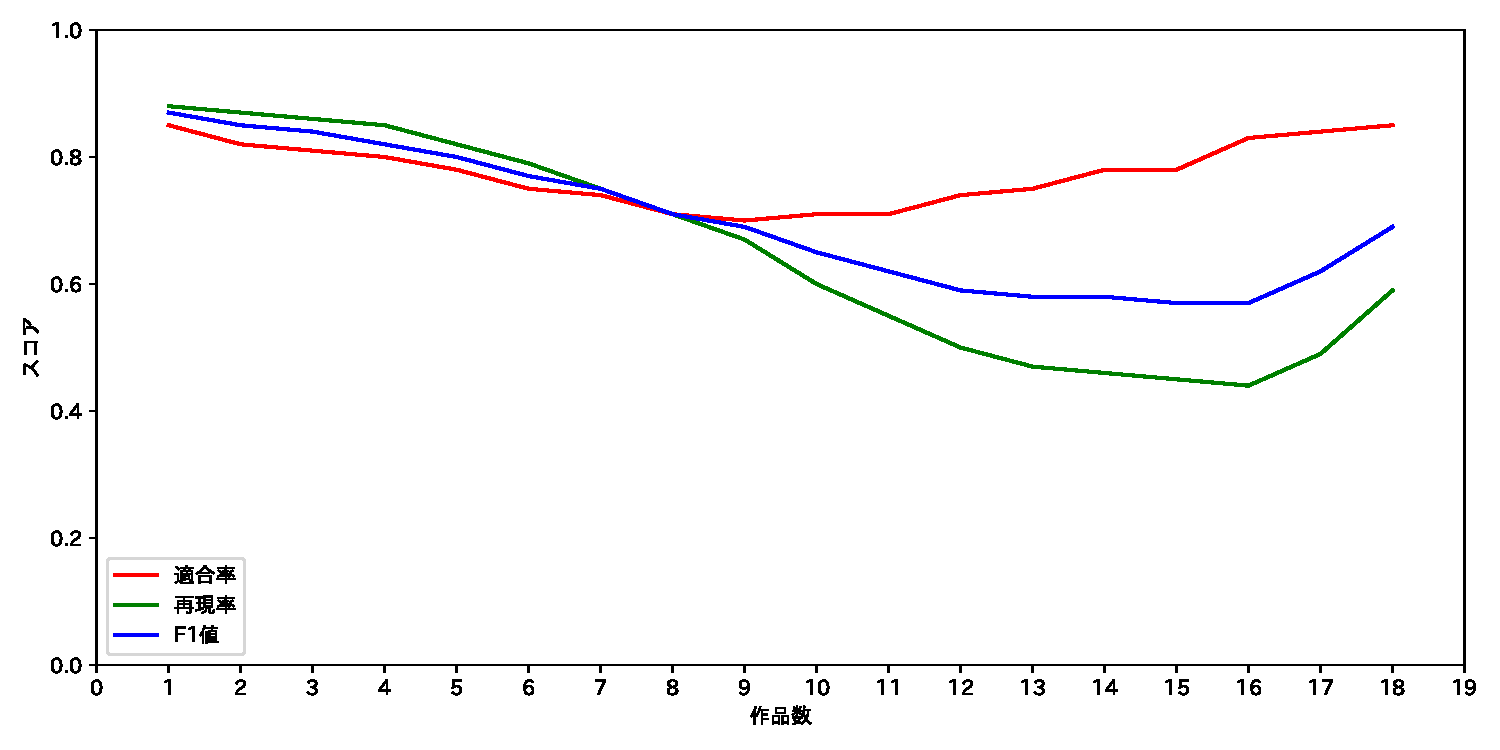
\includegraphics[width=1.0\linewidth]{Okamoto_fig/btod-lines2.pdf}
	\caption{提案BtoDモデルの作品数ごとの評価指標の遷移}
	\label{fig:btod-lines}
 \vspace{-2mm}
\end{figure}

\begin{table}[t]
  \caption{従来BtoDモデルと提案BtoDモデル(L=1)の精度比較}
  \label{tab:btod-model-comp}
  \vspace{1mm}
  \centering
  \scalebox{0.85}{
  \begin{tabular}{l|c|c|c|c}
    \hline\hline
     & 適合率 & 再現率 & F1値 & \begin{tabular}[c]{@{}c@{}}誤予測したユーザ数\end{tabular}\\
    \hline
    従来BtoD & 0.84 & 0.86 & 0.85 & 370\\
    \hline
    提案BtoD(L=1)& \textbf{0.85} & \textbf{0.88} & \textbf{0.87}  & 315\\
    \hline
  \end{tabular}
  }
   \vspace{-2mm}
\end{table}


\begin{figure}[t]
	\centering
	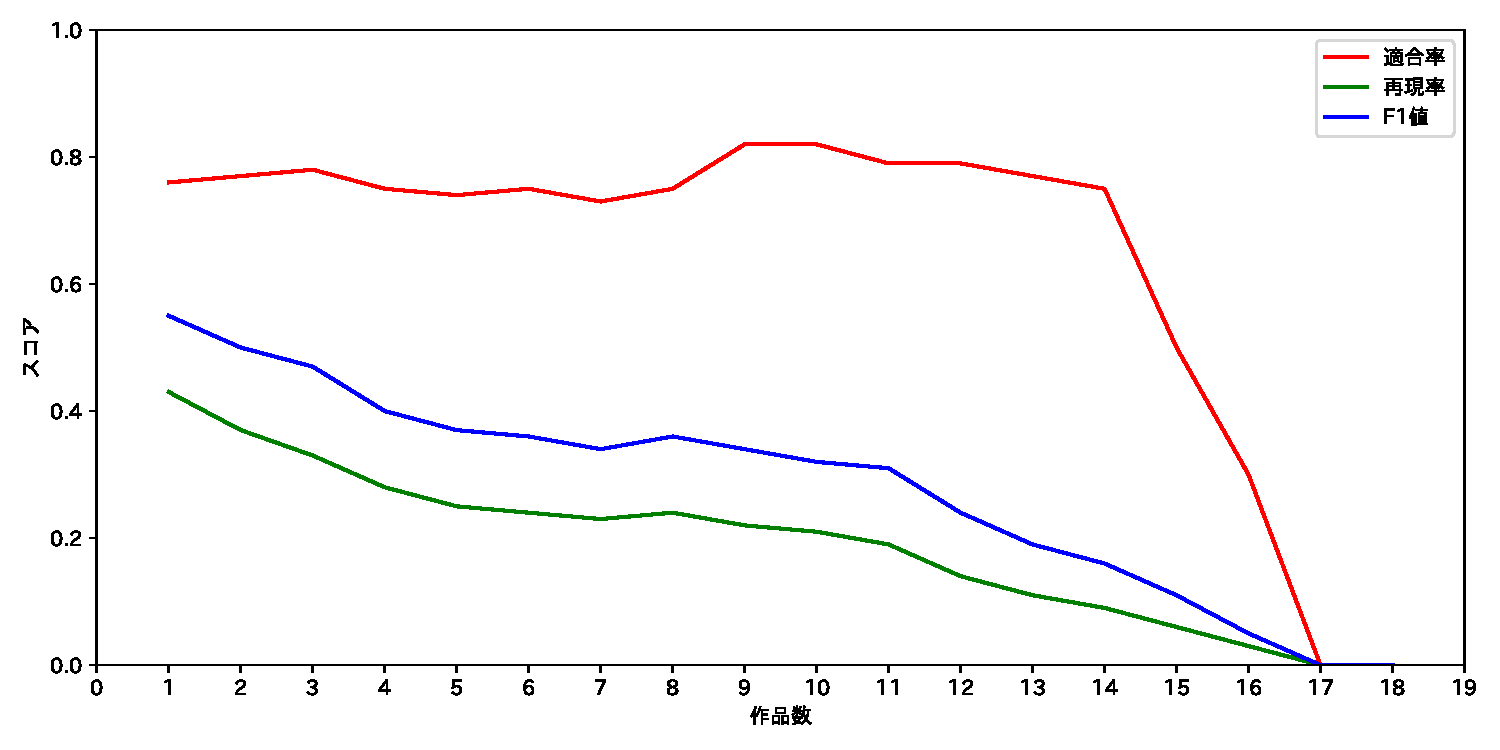
\includegraphics[width=1.0\linewidth]{Okamoto_fig/dtom-lines2.pdf}
	\caption{提案DtoMモデルの作品数ごとの評価指標の遷移}
	\label{fig:dtom-lines}
  \vspace{-2mm}
\end{figure}

\begin{table}[t]
  \caption{従来DtoMモデルと提案DtoMモデル(L=1)の精度比較}
  \label{tab:dtom-model-comp}
  \vspace{2mm}
  \centering
  \scalebox{0.85}{   
  \begin{tabular}{l|c|c|c|c}
    \hline\hline
     & 適合率 & 再現率 & F1値 & \begin{tabular}[c]{@{}c@{}}誤予測したユーザ数\end{tabular}\\
    \hline
    従来DtoM & 0.70 & \textbf{0.44} & 0.54 & 207 \\
    \hline
    提案DtoM(L=1) & \textbf{0.79} & \textbf{0.44} & \textbf{0.57} & 144 \\
    \hline
  \end{tabular}
  }
   \vspace{-2mm}
\end{table}


\begin{table*}[t]
    \caption{従来BtoDモデルと提案BtoDモデル(L=1)における重要度の高い説明変数3件}\label{tab:feature_importance-btod}
    \centering
    \scalebox{0.82}{
        \begin{tabular}{r|rp{60mm}|rp{60mm}}
            \hline\hline
            & \multicolumn{2}{c|}{従来BtoDモデル} & \multicolumn{2}{c}{提案BtoDモデル(L=1)} \\ \cline{2-5}
            グループ & \begin{tabular}{r} 重要度 \end{tabular} & \begin{tabular}{c} 説明変数 \end{tabular} & \begin{tabular}{r} 重要度 \end{tabular} & \begin{tabular}{c} 説明変数 \end{tabular} \\ \hline 
            1 & \begin{tabular}{r}0.05\end{tabular} & \begin{tabular}{r} \{オリジナル/フロー制御/0点\} \end{tabular} & \begin{tabular}{r} 0.20 \end{tabular} & \begin{tabular}{l} \{パス遷移確率P_{n-1,n} \} \end{tabular} \\ \hline
            2 & \begin{tabular}{r} 0.04 \end{tabular} & \begin{tabular}{r} \{リミックス/抽象化/0点\} \end{tabular} & \begin{tabular}{r} 0.04 \end{tabular} & \begin{tabular}{l} \{リミックス/データ表現/0点\} \end{tabular} \\ \hline
            3 & \begin{tabular}{r} 0.04 \end{tabular} & \begin{tabular}{r} \{オリジナル/データ表現/0点\} \end{tabular} & \begin{tabular}{r} 0.03 \end{tabular} & \begin{tabular}{l} \{オリジナル/ユーザ対話性/0点\} \end{tabular} \\ \hline
        \end{tabular}
        }
    \vspace{3mm}

    \caption{従来DtoMモデルと提案DtoMモデル(L=1)における重要度の高い説明変数3件}\label{tab:feature_importance-dtom}
    \centering
    \scalebox{0.82}{
        \begin{tabular}{r|rp{60mm}|rp{60mm}}
            \hline\hline
            & \multicolumn{2}{c|}{従来DtoMモデル} & \multicolumn{2}{c}{提案DtoMモデル(L=1)} \\ \cline{2-5}
            グループ & \begin{tabular}{r} 重要度 \end{tabular} & \begin{tabular}{c} 説明変数 \end{tabular} & \begin{tabular}{r} 重要度 \end{tabular} & \begin{tabular}{c} 説明変数 \end{tabular} \\ \hline 
            1 & \begin{tabular}{r} 0.04 \end{tabular} & \begin{tabular}{l} \{オリジナル/データ表現/0点\} \end{tabular} & \begin{tabular}{r} 0.12 \end{tabular} & \begin{tabular}{l} \{パス遷移確率P_{n-1,n}\} \end{tabular} \\ \hline
            2 & \begin{tabular}{r} 0.04 \end{tabular} & \begin{tabular}{r} \{オリジナル/抽象化/0点\} \end{tabular} & \begin{tabular}{r} 0.05 \end{tabular} & \begin{tabular}{l} \{オリジナル/同期/2点\} \end{tabular} \\ \hline
            3 & \begin{tabular}{r} 0.03 \end{tabular} & \begin{tabular}{r} \{オリジナル/同期/2点\} \end{tabular} & \begin{tabular}{r} 0.04 \end{tabular} & \begin{tabular}{l} \{オリジナル/抽象化/0点\} \end{tabular} \\ 
            \hline
        \end{tabular}
    }
    \vspace{-4mm}
\end{table*}

図\ref{fig:btod-lines}は,BtoDモデルにおいて予測時から遡る作品数$L$別の予測結果(適合率,再現率,F1値)を示す.横軸は作品数$L$,縦軸は各予測評価値を示す.各分類精度は,層化10分割交差検証により出力した10回分の精度の平均値を表している.BtoDモデルの評価指標はノード数$L=1$のときに最も高いF1値となり,適合率は0.85,再現率は0.88,F1値は0.87であった.表\ref{tab:btod-model-comp}は従来BtoDモデルと提案BtoDモデル($L=1$)の予測結果,正しく予測されたBtoDユーザ数,非BtoDユーザと誤予測したBtoDユーザ数を示す.従来手法に比べてわずかに高い精度で予測することができた.具体的には,従来手法でDeveloping以上に到達したユーザ55人(=370人-315人)の誤分類が提案BtoDモデルによって減少した.したがって,Developingに到達する直前に制作する作品で,共通のCT概念を使用する作品を制作していることが示唆される.

図\ref{fig:dtom-lines}は,BtoDモデルと同じ形式でDtoMモデルの結果を示す.DtoMモデルの評価指標はノード数$L=1$のときに最も高いF1値となり,適合率は0.79,再現率は0.44,F1値は0.57であった.表\ref{tab:btod-model-comp}は従来BtoDモデルと提案BtoDモデル($L=1$)の予測結果を示す.従来手法に比べて高い精度で予測することができた.具体的には,従来手法でDeveloping以上に到達したユーザ63人(=207人-144人)の誤分類が提案DtoMモデルによって減少した.したがって,Masterに到達するユーザと到達しないユーザは直前に制作する作品で,共通のCT概念を使用する作品を制作していることが示唆される.



表\ref{tab:feature_importance-btod}と表\ref{tab:feature_importance-dtom}はそれぞれ従来BtoDモデルと提案BtoDモデル,従来DtoMモデルと提案DtoMモデルにおいて,予測精度に寄与した説明変数の結果を示す.重要度の値は,層化10分割交差検証により出力した10回分の重要度の平均値を示す.また,予測精度に寄与する説明変数はCT概念の場合,\{作品の種類/CT概念,点数\}のように示す.BtoDモデル,DtoMモデルは,いずれも本研究で提案する説明変数\{遷移確率$P_{m-1,m}$\}が予測精度に最も寄与しており,特定の習熟度に到達する直前の作品で使用するCTスコアが予測に有用であることが明らかとなった.


\subsubsection{N階マルコフ連鎖モデル}\label{sec:markovResult}

図\ref{fig:markov-btod}は,それぞれ階数N毎のBtoDモデルとDtoMモデルの分類精度(適合率,再現率,F1値)を折れ線グラフで,\ref{sec:marcov-approach}項で述べたとおり予測対象となるユーザが過去に制作した作品のCTパスが学習データに含まれていないため予測できなかったユーザ数(灰色),予測できたが不正解だったユーザ数(青色),予測できて正解したユーザ数(橙色)をそれぞれ積み上げ棒グラフで示す.折れ線グラフの縦軸(左)は予測評価値,積み上げ棒グラフの縦軸(右)はユーザ数,横軸はN階マルコフ連鎖モデルの階数Nを表す.各評価指標は,層化10分割交差検証により出力した10回分の精度の平均値を表し,ユーザ数は層化10分割交差検証により出力した10回分のユーザ数の合計を表している.

図\ref{fig:markov-btod}より,BtoDモデルの評価指標は階数が大きくなるにつれてF1値は向上した.また,DtoMモデルでは階数の大きさに伴いわずかにF1値が向上する程度で,階数が$N=8$のときにF1値が最高値($0.65$)であった.本手法は,従来手法では特定の習熟度に到達するまでのCTパスを考慮していなかったことが原因で誤予測していたユーザの習熟度到達予測を改善する一方で,階数が大きくなるほど予測できるユーザ数が減少することは今後の課題である.

%---------------------
\begin{figure*}[t]
	\centering
	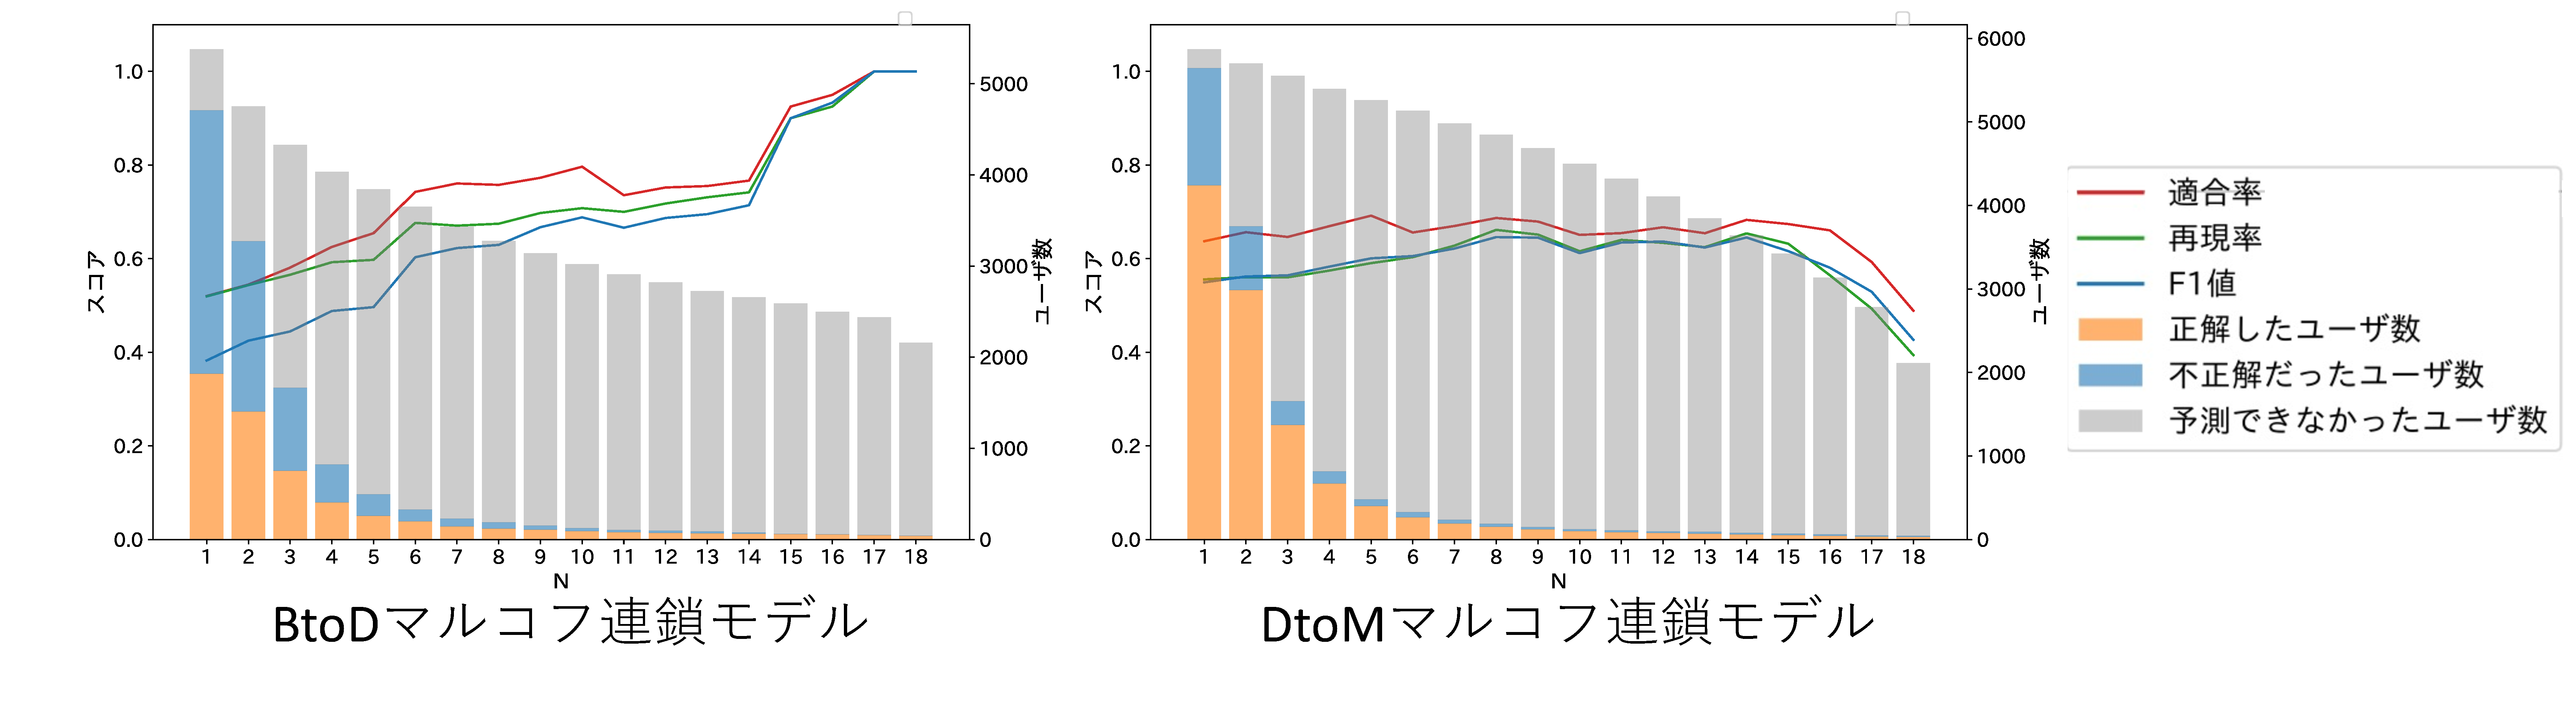
\includegraphics[width=0.9\linewidth]{Okamoto_fig/markov-result.pdf}
        \vspace{-5mm}
	\caption{階数N毎のBtoDマルコフ連鎖モデルの精度とユーザ数の分布}
	\label{fig:markov-btod}
 \vspace{-4mm}
\end{figure*}
%---------------------

\vspace{-5mm}
\subsection{考察}

\subsubsection{予測精度に起因する要因}

\ref{sec:randResult}項で示した通り,2種類のランダムフォレストモデルでは予測する作品から遡る作品数が1つ($L=1$)の時に予測評価値が最も高く,また\ref{sec:markovResult}項では階数が小さいほどより多くのユーザに対して予測することが可能であることを確認した.したがって,特定の習熟度に到達するユーザと到達しないユーザ間では,作品$n-1$から作品$n$へのCTパス重複数に違いがあることが示唆される.図\ref{fig:add-btod}はそれぞれ特定の習熟度に到達したユーザ(BtoDユーザ,またはDtoMユーザ)と到達しなかったユーザ(非BtoDユーザ,または非DtoMユーザ)におけるCT重複数の分布を示す.BtoDユーザは非BtoDユーザよりもCTパス重複数が多く,それぞれの中央値は7.0と3.0であり,Mann–Whitney U検定(p値$<$0.05)によって統計的有意差があることを確認した.一方で,DtoMユーザは非DtoMユーザに比べてCTパス重複数が低く,それぞれ中央値はそれぞれ2.0と4.0であり統計的有意差があることを確認した.

BtoDユーザはRQ1で習熟度Developingに到達するまでに制作した作品で使用するCT概念に共通性が存在することを明らかにしていることもあり,習熟度Developingに到達する直前の遷移確率を使用することで予測精度が向上したことが示唆される.一方で,RQ1でDtoMユーザはBtoDユーザに比べて多様なCTパスを経由して習熟度Masterに到達しているため,習熟度Developingに到達する直前の遷移確率は低いが,到達できない作品の遷移確率が高いため,非DtoMユーザを正しく分類できた結果精度が向上したことが示唆される.

%---------------
\begin{figure}[t]
	\centering
	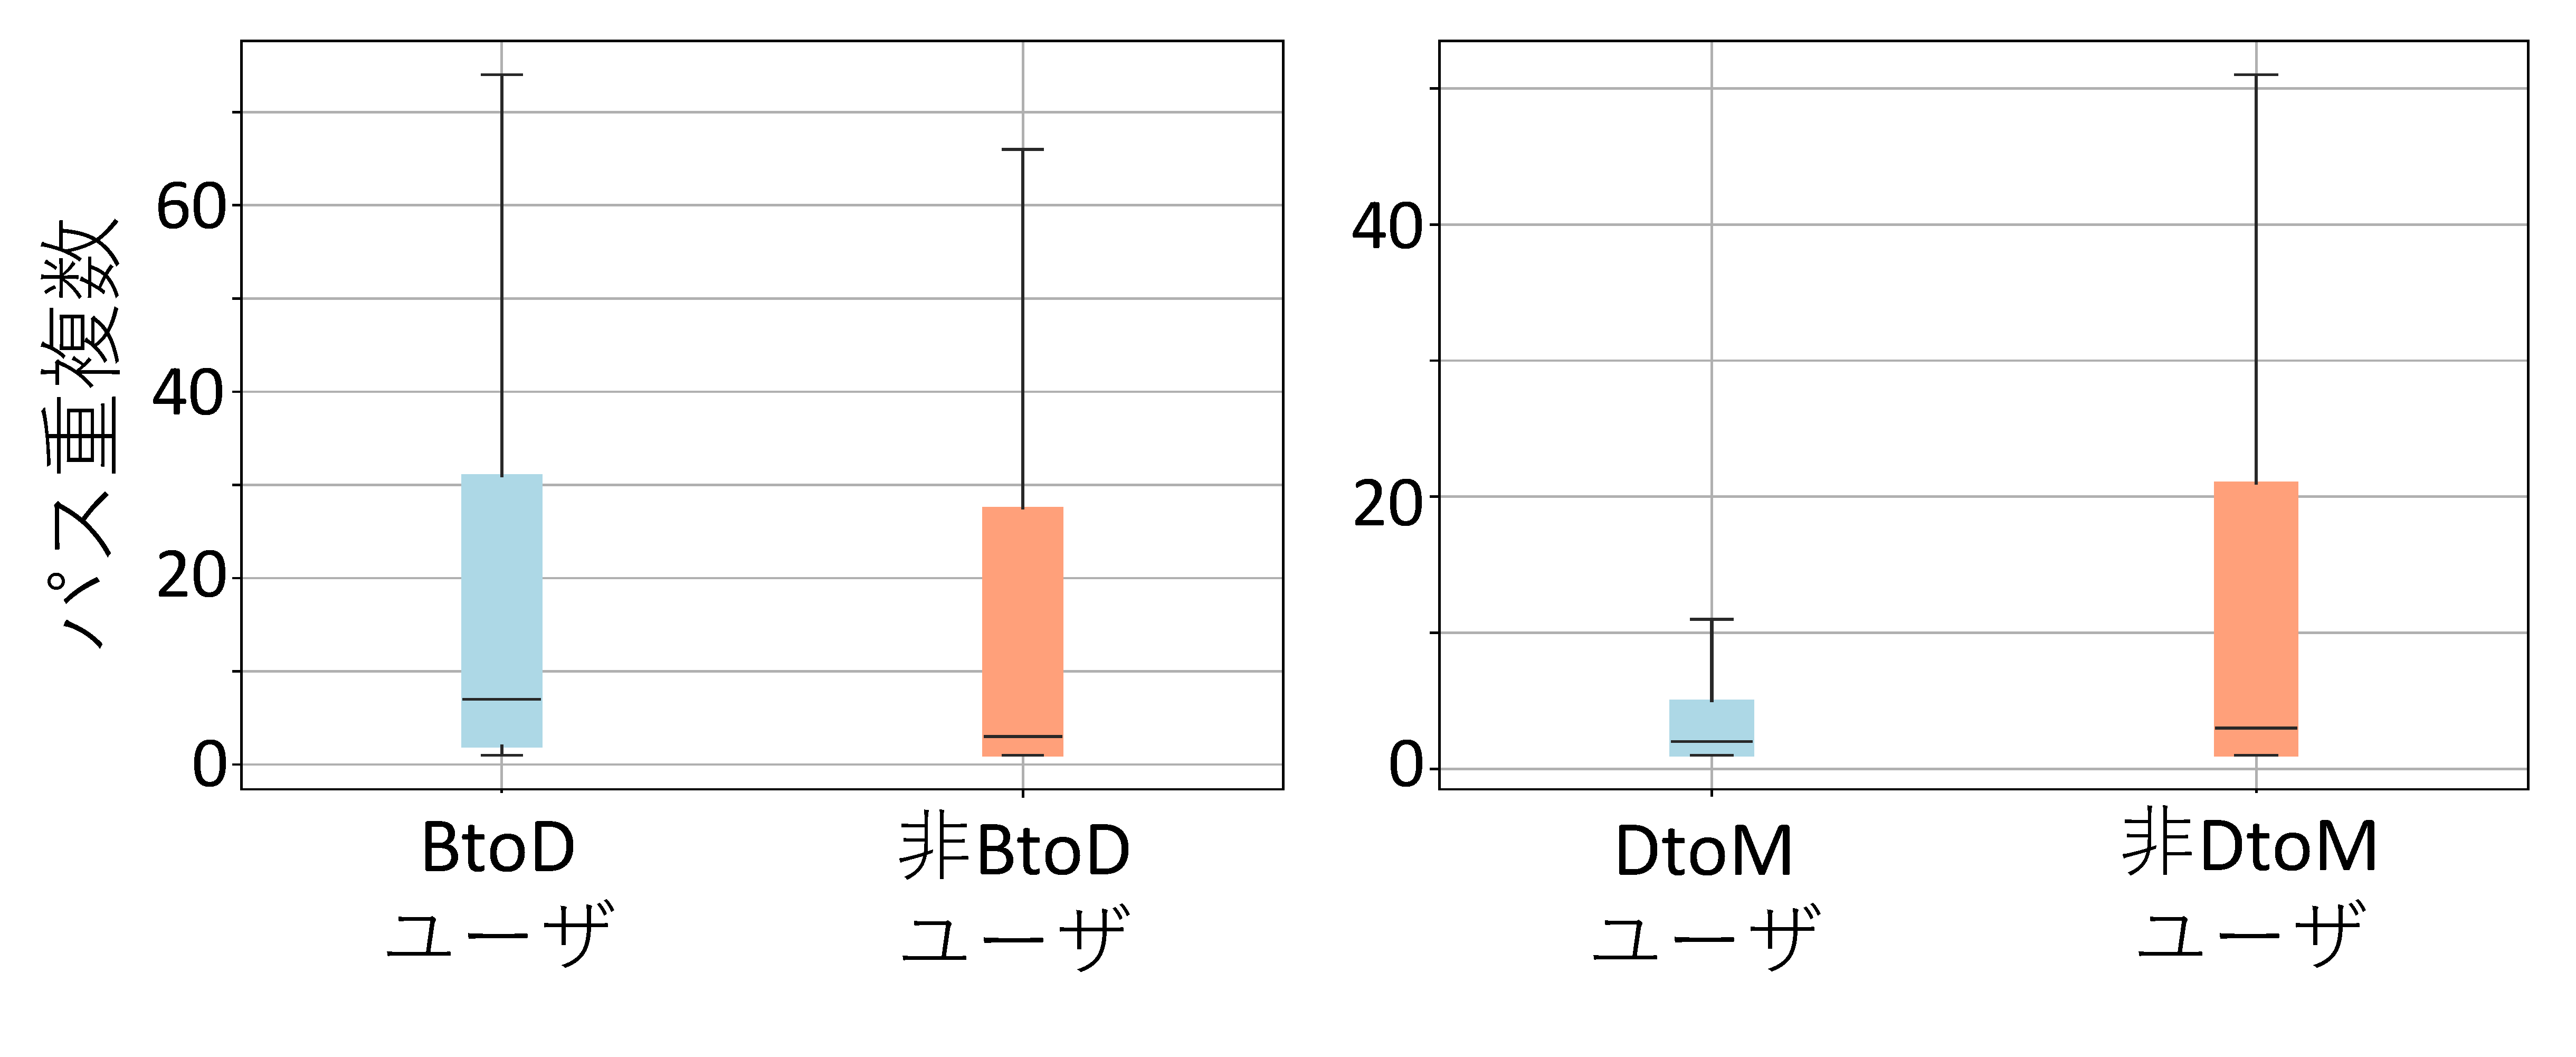
\includegraphics[width=1\linewidth]{Okamoto_fig/add-btod-dtom.pdf}
        \vspace{-7mm}
	\caption{BtoDユーザが直前の作品を制作する前のCTパス重複数}
	\label{fig:add-btod}

 \centering
	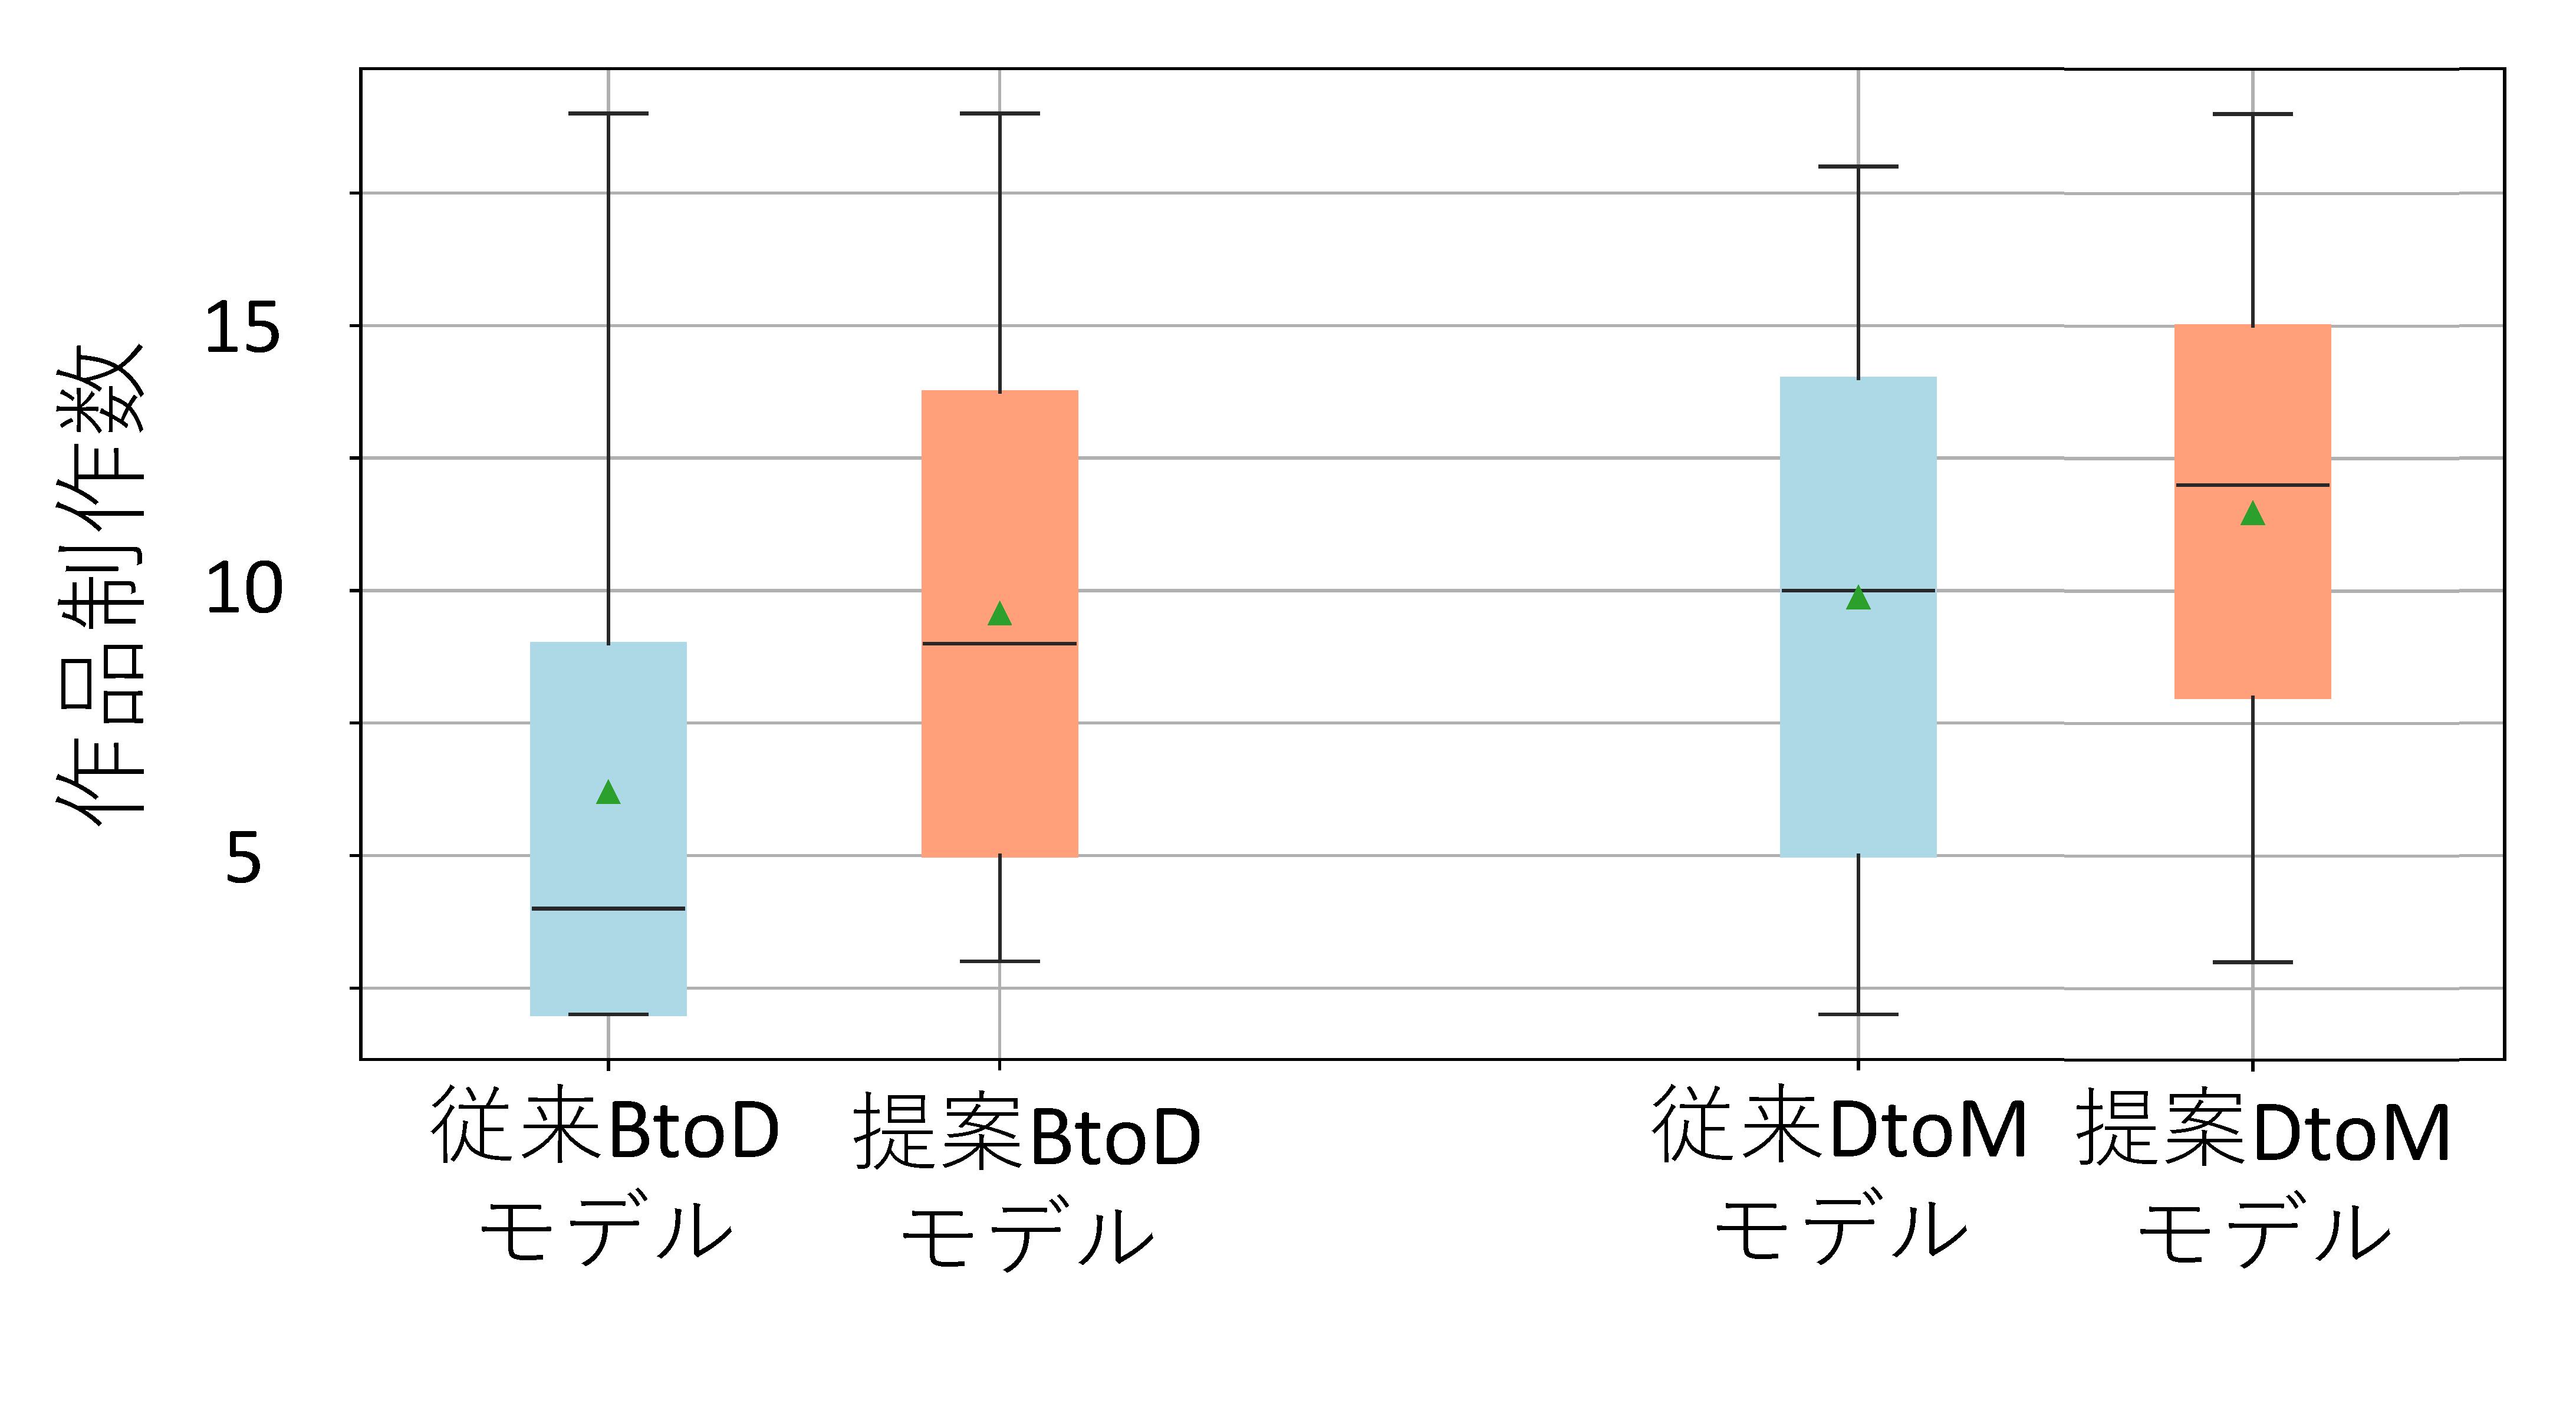
\includegraphics[width=0.75\linewidth]{Okamoto_fig/btod-dtom-path.pdf}
        \vspace{-4mm}
	\caption{従来モデルで予測できたユーザと提案マルコフ連鎖モデルで予測できたユーザの作品制作数の分布}
	\label{fig:btod-path}
\end{figure}
%---------------

% \subsection{従来モデルと提案モデルで予測できたユーザと予測できなかったユーザの特徴分析}
\subsubsection{提案モデルによる貢献可能なユーザ}

本研究が提案したモデルは,従来手法に比べて高い精度で予測できる手法であった.その理由を明らかにするために,本研究の提案手法と従来手法において,正確に予測したユーザの特徴の違いを調査する.図\ref{fig:btod-path}は従来モデルで正確に予測できた正クラスのユーザ(BtoDユーザまたはDtoMユーザ)とN階マルコフ連鎖モデルのみで正確に予測できた正クラスのユーザが制作した作品数の分布を示す.BtoDモデル,DtoMモデルともにN階マルコフ連鎖モデルが従来モデルよりもより作品制作数の多いユーザの予測に成功しており,いずれもMann–Whitney U検定(p値$<$0.05)によって統計的有意差があることを確認した.したがって,本研究が提案するN階マルコフ連鎖モデルは作品制作数の多いユーザの予測に有用である一方で,作品制作数の少ないユーザは従来手法を利用する方が良いことが示唆される.

表\ref{tab:path-btod}は,従来モデルでCT概念の獲得有無のみを学習していたため誤分類されたが,N階マルコフ連鎖モデルで正しく予測されたユーザ1人を抽出し,作品のCTスコアを制作順に示す.当該ユーザはリミックス作品を制作した直後に類似のCT概念を使用したオリジナル作品を制作している.具体的には1作品目と2作品目,3作品目と4作品目,7作品目と8作品目が該当する.他のユーザでも同じような傾向が見られた.このような作品制作順序に特徴を持つ場合は,N階マルコフ連鎖モデルが有用であることが示唆される.

例えば,3作品目のリミックス作品を制作した直後の4作品目では全く同じCT概念を持つ作品を制作している.点数は若干異なるが,1,2作品目,7,8作品目でも同じような傾向が見られる.また,他にも数件このようなケースが見られたため,本モデルはRQ1のBtoDユーザのCTスキル習熟過程の分析結果で得られたような,繰り返し同じCT概念の作品を制作するユーザの特徴を捉え,予測が可能になっていることが示唆された.

また,本研究ではN階マルコフ連鎖モデルの階数Nを大きくすると予測できないユーザ数が増加して汎用性が低下したが,これは説明変数の7つのCT概念を完全一致によって判定しているためであり,CT概念の部分一致に基づき予測することで汎用性を高めることができると考える.

\begin{table}[t]
    \centering
    \caption{N階マルコフ連鎖モデルで予測が成功し,従来手法で誤予測したBtoDユーザの作品制作過程}
    \label{tab:path-btod}
    \vspace{3mm}
    \scalebox{0.85}{
      \begin{tabular}{c|c|cccccccc}
\hline\hline
\multirow{2}{*}{制作順序} & \multicolumn{1}{l|}{\multirow{2}{*}{\small{リミックス}}} & \multicolumn{8}{c}{CTスコア}                                                                                                                                                         \\ \cline{3-10} 
                    & \multicolumn{1}{l|}{}                       & \multicolumn{1}{c|}{A} & \multicolumn{1}{c|}{P} & \multicolumn{1}{c|}{L} & \multicolumn{1}{c|}{S} & \multicolumn{1}{c|}{F} & \multicolumn{1}{c|}{U} & \multicolumn{1}{c|}{D} & 合計 \\ \hline 
1                   & 1                                           & \multicolumn{1}{c|}{1} & \multicolumn{1}{c|}{0} & \multicolumn{1}{c|}{0} & \multicolumn{1}{c|}{1} & \multicolumn{1}{c|}{1} & \multicolumn{1}{c|}{2} & \multicolumn{1}{c|}{1} & 6  \\ \hline
2                   & 0                                           & \multicolumn{1}{c|}{1} & \multicolumn{1}{c|}{1} & \multicolumn{1}{c|}{0} & \multicolumn{1}{c|}{1} & \multicolumn{1}{c|}{2} & \multicolumn{1}{c|}{1} & \multicolumn{1}{c|}{1} & 7  \\ \hline
3                   & 1                                           & \multicolumn{1}{c|}{1} & \multicolumn{1}{c|}{1} & \multicolumn{1}{c|}{0} & \multicolumn{1}{c|}{1} & \multicolumn{1}{c|}{2} & \multicolumn{1}{c|}{1} & \multicolumn{1}{c|}{1} & 7  \\ \hline
4                   & 0                                           & \multicolumn{1}{c|}{1} & \multicolumn{1}{c|}{1} & \multicolumn{1}{c|}{0} & \multicolumn{1}{c|}{1} & \multicolumn{1}{c|}{2} & \multicolumn{1}{c|}{1} & \multicolumn{1}{c|}{1} & 7  \\ \hline
5                   & 0                                           & \multicolumn{1}{c|}{1} & \multicolumn{1}{c|}{2} & \multicolumn{1}{c|}{0} & \multicolumn{1}{c|}{0} & \multicolumn{1}{c|}{1} & \multicolumn{1}{c|}{2} & \multicolumn{1}{c|}{1} & 7  \\ \hline
6                   & 0                                           & \multicolumn{1}{c|}{1} & \multicolumn{1}{c|}{1} & \multicolumn{1}{c|}{0} & \multicolumn{1}{c|}{1} & \multicolumn{1}{c|}{1} & \multicolumn{1}{c|}{1} & \multicolumn{1}{c|}{1} & 6  \\ \hline
7                   & 1                                           & \multicolumn{1}{c|}{1} & \multicolumn{1}{c|}{3} & \multicolumn{1}{c|}{0} & \multicolumn{1}{c|}{3} & \multicolumn{1}{c|}{2} & \multicolumn{1}{c|}{1} & \multicolumn{1}{c|}{1} & 11  \\ \hline
8                   & 0                                           & \multicolumn{1}{c|}{1} & \multicolumn{1}{c|}{3} & \multicolumn{1}{c|}{0} & \multicolumn{1}{c|}{3} & \multicolumn{1}{c|}{1} & \multicolumn{1}{c|}{1} & \multicolumn{1}{c|}{1} & 10  \\ \hline
\end{tabular}
}
  \end{table}

%%%%%%%%%%%%%%%%%%%%%%%%%%
\section{おわりに}\label{sec:conc}
%%%%%%%%%%%%%%%%%%%%%%%%%%

本研究では,特定の習熟度に到達するまでの過程で使用したCTスキル,および各CTスキルを用いたユーザの作品制作数を分析し,習熟度を予測するモデルを構築した.提案するモデルは従来手法よりも高い精度でユーザの習熟度を予測できることを確認した.今後は,マルコフ連鎖モデルの状態の部分一致による汎用性を高める方法を検討し,ScratchにおけるユーザのCTスキル獲得状況に合わせた作品推薦に取り組む.

\bibliographystyle{junsrt}
\bibliography{Okamoto}

\end{document}



